\chapter{Erstellung der Computerspielengines}
\label{chapter:erstellung-der-computerspielengines}

Nachdem Patchwork auf unterschiedlichste Aspekte analysiert und das Brettspiel als Computerprogramm umgesetzt wurde, werden nachfolgend die verschiedenen Computerspielengines für das Spiel implementiert.

\section{Ansatz A: Zufallsauswahl der Spielzüge}
\label{section:erstellung-ansatz-a}

Um eine Computerspielengine zu erstellen, muss das Trait \code{Player}, welcher in Codeausschnitt \ref{code:player-trait} zu sehen ist, von der Engine implementiert werden. Dafür müssen die zwei Methoden \code{name()} und \code{get\_action()} implementiert werden. Die erste Methode gibt den Namen der Computerspielengine zurück, um sie während des Spiels identifizieren zu können, während die zweite Methode die Aktion als \code{PlayerResult<Action>} zurückgibt, die der Spieler machen möchte und benötigt als Eingabe den aktuellen Zustand des Spiels.

\lstinputlisting[
    label={code:player-trait},
    caption={Definition des Player-Traits},
    captionpos=b,
    language=Rust,
    firstline=0,
]{res/code/player-trait.rs}

Die einfachste Computerspielengine ist der \code{RandomPlayer}, in Codeauschnitt \ref{code:random-player} zu sehen, welcher einen Spieler repräsentiert, der zufällige Züge macht. Zur Auswahl der Züge verwendet die Engine den Zufallsgenerator Xoshiro256++, der einen der möglichen Spielzüge im aktuellen Spielzustand \code{game} auswählt, die durch den Aufruf der Methode \code{game.get\_valid\_actions()} bereitgestellt werden. Dieser Computergegner ist gut für Vergleichszwecke im späteren Kapitel \nameref{chapter:evaluation} geeignet, da die zufälligen Züge eine Baseline gegen die komplexeren, strategischen Entscheidungen der anderen Computerspielengines bildet.

\lstinputlisting[
    label={code:random-player},
    caption={Definition des RandomPlayers},
    captionpos=b,
    language=Rust,
    firstline=0,
]{res/code/random-player.rs}

\pagebreak

\section{Ansatz B: Greedy-Algorithmus}

Die Computerspielengine, welche mit dem Greedy-Algorithmus arbeitet, ist ebenfalls ein weiterer guter Vergleichskandidat für die komplexeren Computergegner. Wenn der Greedy-Algorithmus vor eine Entscheidung gestellt wird, wählt dieser immer den Spielzug, der in der aktuellen Situation optimal erscheint, auch wenn der Spielzug sich im weiteren Spielverlauf nicht als bester Zug herausstellt \cite[S. 234]{2023Greedy}. Durch die direkte Bewertung mittels des Evaluators mit 1-Zug-Voraussicht ist dieses zukünftige Wissen allerdings nicht bekannt. Als einer der Evaluatoren wurde für diesen Computergegner eine \enquote{Handcrafted Evaluation} implementiert. Dieser Evaluator zeichnet sich dadurch aus, dass er zahlreiche Heuristiken und Regeln verwendet, um eine Evaluierung einer Position zu determinieren \cite{2023.StockfishTerminology}.

\lstinputlisting[
    label={code:evaluator},
    caption={Evaluierer für den Spielzustand},
    captionpos=b,
    language=Rust,
    firstline=0,
]{res/code/evaluator.rs}

\pagebreak

Um einen Evaluator zu erstellen, muss der Trait \code{Evaluator} implementiert werden. Dieser ist in Codeausschnitt \ref{code:evaluator} zu sehen und beinhaltet drei Methoden. Tatsächlich muss jedoch nur die erste Methode \code{evaluate\_intermediate\_node()} implementiert werden, da die anderen beiden Methoden \code{evalute\_terminal\_node()} und \code{evaluate\_node()} allgemeingültige Standardimplementierungen besitzen. Die Methoden funktionieren alle gleich: Sie nehmen den aktuellen Spielzustand an und geben dann eine Zahl aus, welche die Evaluierung der Position beschreibt, wobei eine große Zahl in negative oder positive Richtung für den jeweiligen Spieler gut ist.

Der \enquote{Handcrafted Evaluator} für diese Computerspielengine, \code{StaticEvaluator} im Quellcode genannt, berechnet wie folgt die Evaluation für die aktuelle Spielposition. Es werden die Scores für beide Spieler berechnet und anschließend die Evaluation gebildet, indem der Score des Gegners von dem Score des Spielers abgezogen wird. Innerhalb der Berechnung des Scores für einen Spieler werden folgende Berechnungsgrundlagen angewandt:

Als erster Faktor wird die Spielposition, die mit den normalen Endregeln berechnet wird, als $es$ eingerechnet. Die normalen Endregeln bedeuten in diesem Fall, dass für jedes freie Feld zwei Punkte abgezogen werden und jeder Knopf, der dem Spieler gehört, mit einem Punkt gewertet wird.

Als zweiter Faktor wird mit $ps$ einberechnet, an welcher Stelle der Zeitstein des Spielers liegt. Für jedes Feld, über das der Zeitstein noch nicht gezogen ist, wird dieser Faktor mit einem Punkt mehr gewertet.

Als dritter Faktor wird die Bewertung des Ablageplans des Spielers $bs$ miteingerechnet. Dazu wird zuerst die Feldanzahl mit neun multipliziert, um immer für $bs$ eine positive Punktzahl zu bekommen. Im Fall von Patchwork mit seinen 81 Felder pro Ablageplan ist somit die initiale Punktezahl 719. Nun wird für jedes freie Feld auf dem Ablageplan neun Punkte von der Punktzahl abgezogen, somit kommt man bei einem komplett leeren Ablageplan auf einen $bs$ von null. Anschließend wird für jedes Feld, auf dem ein Teil von einem Flicken liegt, berechnet wie viele leere Nachbarfelder dieses hat und für jedes leere Feld ein Punkt abgezogen. Der Rand gilt bei dieser Berechnung als befülltes Feld, wenn er als Nachbarfeld in Frage kommt, für den Rand werden jedoch nicht die leeren Nachbarfelder bestimmt.

\pagebreak

Zur Bestimmung, was die Nachbarn eines Feldes sind, gibt es zwei klassische Nachbarschaften: Die von Neumann Nachbarschaft, wobei alle Felder als Nachbar gelten, welche eine Manhattan-Distanz entfernt sind und die Moore Nachbarschaft, bei der alle Felder als Nachbar gelten, die eine Tschebyscheff-Distanz entfernt sind \cite[S. 2]{2016.kneighborhood}. In der Abbildung \ref{fig:nachbarschaften} sind diese beiden Nachbarschaften grafisch dargestellt und jeweils mit zwei Beispielen im Patchwork-Kontext versehen. Für die Implementierung der Nachbarschaft wurde sich für die Moore Nachbarschaft entschieden, um alle umliegenden Felder des betrachten Feld abzudecken.

\vspace*{-0.25cm}
\begin{figure}[!ht]
    \centering
    \includegraphics[width=\textwidth]{res/pictures/nachbarschaften.pdf}
    \vspace*{-0.45cm}
    \caption{Mögliche Nachbarschaften für den Evaluator}
    \label{fig:nachbarschaften}
\end{figure}
\vspace*{-0.2cm}

Als vierter Faktor wird der Knopfeinkommen-Score $bis$ miteingerechnet. Die Formel \ref{eqn:button-income-score} zur Berechnung dieses Scores benötigt die Argumente $tp$ und $bi$, wobei das erste Argument die Anzahl der schon überschrittenen Knopfwertungen beschreibt und das zweite Argument die Höhe des Knopfeinkommen vom Spieler beschreibt, also wie viele Knöpfe dieser bei Überschreiten einer Knopfwertung erhält. Je weniger Knopfwertungen vor dem Zeitstein des Spielers sind, desto weniger Nutzen besitzt eine hohes Knopfeinkommen. Daher bewertet dieser Score die untenstehende Formel mit exponentiellem Zerfall. Wurde noch kein Knopfeinkommen überschritten, so bringt jeder Knopf des Knopfeinkommens acht Punkte, wohingegen nur noch ein Punkt pro Knopf im Knopfeinkommen gewertet wird, wenn noch ein Knopfwertung aussteht.

\begin{equation}
    \label{eqn:button-income-score}
    bis(tp, bi) = 8 \cdot e^{\frac{tp}{8}\ln\left(\frac{1}{8}\right)} \cdot bi
\end{equation}

Um die Evaluation für eine Spielposition zu erhalten, werden mit der folgenden Formel \ref{eqn:evaluator-score} alle Faktoren zusammengerechnet. $\tau$ beschreibt hierbei als Prozentzahl, wie weit das Spiel der Spielposition schon fortgeschritten ist. Daraus lässt sich schließen, dass zu Beginn eines Spiels der Ablageplan-Score $bs$ im Verhältnis zum Endscore $es$ viel höher gewichtet wird, um statt viele Felder mit Flicken zu befüllen, die Flicken sinnvoll platziert werden, zum Beispiel am Rand oder nahtlos anschließend an andere Flicken. Beide Faktoren werden zweifachgewichtet in die Evaluation mit einberechnet, während der Positions-Score für den Zeitstein $ps$ und der Knopfeinkommen-Score $bis$ nur einfach gewichtet sind. Diese Gewichtung wurde vorgenommen, um möglichst viele Strafpunkte pro freies Feld auf dem Ablageplans zu vermeiden und in beide vorderen Scores der Ablageplan von großer Bedeutung ist.

\begin{equation}
    \label{eqn:evaluator-score}
    eval = 2 \cdot bs \cdot (1 - \tau) + 2 \cdot es \cdot \tau + ps + bis
\end{equation}

Neben dem \enquote{Handcrafted Evaluator} gibt es noch zwei weitere Evaluatoren. Der Win-Loss-Evaluator lässt zur Bewertung einer Spielposition das Spiel von dieser Stelle aus zufällig zu Ende spielen und gibt dann eine 1 zurück, wenn Spieler 1 gewonnen hat und eine -1, falls der zweite Spieler in dem zufälligen Spielende gewonnen hat. Somit entspricht dieser Evaluator der Simulationsphase innerhalb einer \ac{MCTS} Iteration. Der Score-Evaluator erweitert den Win-Loss-Evaluator insofern, dass auch die bei Patchwork entstehenden Endergebnisse berücksichtigt werden, \dash auch hier wird von der Position zufällig bis zum Ende gespeilt, mit dem einzigen Unterschied, dass am Ende nicht -1 oder 1 zurückgegeben wird, sondern die Differenz der Endwertung der beiden Spieler.

\pagebreak

\section{Ansatz C: Principal-Variation-Search}
\label{section:erstellung-ansatz-b}

Der dritte und erste richtige Versuch eines starken Computerspielgegners ist der \acl{PVS} Spieler. Für das Finden der besten Aktion verwendet der \acs{PVS} Spieler dabei eine optimierte Variante des Alpha-Beta-Suchalgorithmus, die \acf{PVS}. Bei der \ac{PVS} werden mehrere Änderungen vorgenommen. Zuerst wird der klassische Minimax-Algorithmus mittels Negamax implementiert. Bei Nullsummenspielen wie Patchwork ist der maximale Wert des einen Spielers immer der negierte minimale Wert des anderen Spielers ($\max\left(a,b\right) = -\min\left(-a,-b\right)$) \cite[S. 9]{2020.MinimaxTheorem}. Bei Negamax wird dies ausgenutzt, indem immer dieselbe Funktion aufgerufen wird und das Ergebnis negiert wird, anstatt zwei verschiedene Fälle für den min- und max-Spieler zu haben. Dies funktioniert aber nur, wenn der aktive Spieler nach jedem Spielzug wechselt. Dies ist in Patchwork nicht der Fall, kann in der Computerspielimplementierung aber erzwungen werden, indem der \code{do\_action} Methode ein \enquote{force player switch} Parameter übergeben wird. Würde der Spieler im Normalfall nicht wechseln, so wird einfach ein Spielerwechsel erzwungen und dem neuen Spieler nur die \emph{Phantom}-Aktion zur Verfügung gestellt. So kann auch die Suche in Patchwork ohne Probleme als Negamax implementiert werden, was die Implementierung vereinfacht. Bei Minimax-basierten Algorithmen wird immer eine Bewertungsfunktion für die Evaluation der Blattknoten benötigt. Hierzu wird der im vorherigen Abschnitt vorgestellte \code{StaticEvaluator} verwendet. Um genauer auf die weiteren Unterschiede von \ac{PVS} im Vergleich zur Alpha-Beta Suche eingehen zu können, müssen zunächst die in der Suche auftretenden Knotentypen erläutert werden:

\vspace*{-0.45cm}

\begin{figure}[!ht]
    \centering
    \includegraphics[width=0.695\textwidth]{res/pictures/minimal-search-tree.pdf}
    \caption{Minimaler Suchbaum bei der Alpha-Beta Suche}
    \label{fig:minimal-search-tree}
\end{figure}

\vspace*{-5cm}

\pagebreak

\begin{itemize}
    \item \labeltext{\emph{\acs{PV}-Knoten}}{text:pv-node} oder \emph{Typ-1-Knoten}: Die \ac{PV} ist eine Sequenz an Aktionen, bei denen beide Spieler immer die für sich beste Aktion wählen. Es handelt es also um den \enquote{perfekten} Spielverlauf, bei dem kein Pruning stattfinden kann. \cite[S. 316f.]{2005.EnhancedForwardPruning}
    \item \vspace*{-0.125cm} \labeltext{\emph{Cut-Knoten}}{text:cut-node} oder \emph{Typ-2-Knoten}: Sind Knoten, bei denen ein $\beta$-Cutoff stattgefunden hat, \dash es gab eine Suche mit den Grenzen $\left[\alpha, \beta\right]$ und der Wert war $\ge \beta$. Somit wurde in diesem Teilbaum für einen Spieler eine Aktion gefunden, die zu gut war, sodass der andere Spieler vorher eine andere Aktion auswählen wird, damit das Spiel überhaupt nicht in den Zustand dieses Knotens kommen kann. \cite[S. 324]{1975.AlphaBeta}
    \item \vspace*{-0.125cm} \labeltext{\emph{All-Knoten}}{text:all-node} oder \emph{Typ-3-Knoten}: Während der Suche aller Kinderknoten wurde kein Spielzustand gefunden, der besser als ein anderer Spielzustand, welchen der aktuelle Spieler durch das Ausführen einer anderen Aktion in einem anderen Teil des Suchbaums erreichen konnte. Bei einer Suche mit Grenzen $\left[\alpha, \beta\right]$ war die Evaluation aller Kinderknoten also $\le \alpha$. \cite[S. 446]{1985.ParallelAlphaBeta}
\end{itemize}

\vspace*{-0.13cm}

Mithilfe dieser Knotentypen lässt sich der minimale für Alpha-Beta-Pruning benötigte Suchbaum aufstellen \cite[S. 8]{1991.SingleAgentGameTreeSearch}. Dieser ist in Abbildung \ref{fig:minimal-search-tree} visualisiert. Da Alpha-Beta als Tiefensuche agiert, werden immer zuerst alle \hyperref[text:pv-node]{\acs{PV} Aktionen / Knoten} durchsucht. Jeder \hyperref[text:pv-node]{\emph{\acs{PV}-Knoten}} hat dabei immer genau einen weiteren \hyperref[text:pv-node]{\emph{\acs{PV}-Knoten}} sowie mehrere \hyperref[text:cut-node]{\emph{Cut-Knoten}} als Kinder. Die \hyperref[text:cut-node]{\emph{Cut-Knoten}} erzeugen dabei einen Teilbaum, bei dem sich immer wieder \hyperref[text:cut-node]{\emph{Cut-Knoten}} und \hyperref[text:all-node]{\emph{All-Knoten}} abwechseln. Bei \hyperref[text:cut-node]{\emph{Cut-Knoten}} muss immer nur das erste Kind durchsucht werden, während bei allen anderen Kinderknoten ein $\beta$-Cutoff stattfinden kann. Bei \hyperref[text:all-node]{\emph{All-Knoten}} müssen immer alle Kinderknoten durchsucht werden.

\acl{PVS} setzt an dieser Stelle an, indem versucht wird den minimalen Suchbaum auch während der Suche zu erhalten. Dazu wird die Alpha-Beta-Suche mit einer iterativen Tiefensuche kombiniert, \dash zuerst wird der gesamte Suchbaum mit Tiefe 1 durchsucht, dann mit Tiefe 2 und so weiter. Dieser Vorgang wiederholt sich, bis die Suchzeit vorbei ist. In jeder Iteration, wird dabei in jeder Ebene die beste gefundene Aktion, die \acl{PV}, gespeichert. In der nächsten Iteration wird dann davon ausgegangen, dass es sich bei der \acl{PV} der vorherigen Suche auch weiterhin um die \acl{PV} handelt, auch wenn nun eine Ebene tiefer gesucht wird. Sollte dies der Fall sein, können sehr große Teilbereiche des Baums schnell geprunt werden. Die iterative \ac{PVS} Tiefensuche ist dabei durch die größere Anzahl an geprunten Knoten im Regelfall schneller als die Alpha-Beta Suche mit einer festen Tiefe \cite[S. 13]{2017.Minimax}.

\begingroup

\setlength{\textfloatsep}{0pt}
\setlength{\intextsep}{0pt}

\refstepcounter{lstlisting}
\addcontentsline{lol}{lstlisting}{\protect\numberline{\thelstlisting}Pseudocode vom Principal-Variation-Search Algorithmus}

\begin{algorithm}[!ht]
    \caption{Pseudocode vom Principal-Variation-Search Algorithmus}
    \label{algo:principal-varation-search}
    \begin{algorithmic}[1]
        \Function{pvs}{$game$,\, $\alpha$,\, $\beta$,\, $depth$}
        \If{$depth == 0$ oder $game$ ist Terminalzustand}
        \State \Return $color\ \cdot $ \Call{evaluation}{$game$} \Comment{$max$-Player $color = 1$, sonst $-1$}
        \EndIf
        \For{each valid $action$ of $game$}
        \State $game.$\Call{do\_action}{$action$}
        \If{$action$ ist erste Aktion} \Comment{$\acs{PV}$-Action}
        \State $value = -$\Call{pvs}{$game$,\, $-\beta$,\, $-\alpha$,\, $depth - 1$} \label{alg:pvs-line-8}
        \Else
        \State $value = -$\Call{pvs}{$game$,\, $-\alpha - 1$,\, $-\alpha$,\, $depth - 1$} \Comment{\small \acf{ZWS}} \label{alg:pvs-line-10}
        \If{$\alpha < value < \beta$}
        \State $value = -$\Call{pvs}{$game$,\, $-\beta$,\, $-\alpha$,\, $depth - 1$} \label{alg:pvs-line-12}
        \EndIf
        \EndIf
        \State $game.$\Call{undo\_action}{$action$}
        \If{$value \ge \beta$}
        \State \Return $\beta$ \Comment{$\beta$-Cutoff}
        \EndIf
        \State $\alpha = \max\left(\alpha, value\right)$ \label{alg:pvs-line-19}
        \EndFor
        \EndFunction
    \end{algorithmic}
\end{algorithm}

\endgroup

In Pseudocode \ref{algo:principal-varation-search} ist die \ac{PVS}-Suche abgebildet. Alle Aktionen werden bei jeden Methodenaufruf so angeordnet, dass die \acl{PV} der vorherigen Suche die erste Aktion ist. Da dort ein \hyperref[text:pv-node]{\emph{\acs{PV}-Knoten}} erwartet wird, findet eine Suche mit dem normalen $\alpha$-$\beta$-Fenster statt (\hyperref[alg:pvs-line-8]{Zeile 8}). In allen anderen Fällen soll so schnell wie möglich bewiesen werden, dass man sich nicht mehr in einem \hyperref[text:pv-node]{\emph{\acs{PV}-Knoten}} befindet. Dazu wird die untere Begrenzung des $\alpha$-$\beta$-Fensters auf die Evaluation gesetzt (\hyperref[alg:pvs-line-19]{Zeile 19}). Handelt es sich bei der ersten Aktion tatsächlich um die \acl{PV}, so müssten alle weiteren Aktionen schlechter sein und somit eine Evaluation $\le \alpha$ zurückgeben. Um dies so schnell wie möglich zu beweisen, wird eine \acf{ZWS}, eine Suche mit einem Fenster $\left[\alpha, \alpha + 1\right]$, ausgeführt (\hyperref[alg:pvs-line-10]{Zeile 10}) \cite[S. 317]{2005.EnhancedForwardPruning}. Dadurch, dass die obere Grenze mit $\alpha + 1$ so niedrig wie möglich ist, werden deutlich mehr $\beta$-Cutoffs produziert als mit dem normalen $\beta$ Parameter. Solange der tatsächliche Wert auch unterhalb von $\alpha$ liegt, stellt das kein Problem dar. Ist diese Annahme falsch, so muss die Suche mit dem normalen $\alpha$-$\beta$-Fenster erneut durchgeführt werden, um die tatsächliche Evaluation des Knotens zu erhalten (\hyperref[alg:pvs-line-12]{Zeile 12}) \cite{2002.PrincipalVariationSearch}. Ist die tatsächliche Evaluation besser als der derzeitige $\alpha$-Wert, so war auch die Annahme, dass die erste Aktion die \acl{PV} ist, falsch und der Knoten wird als die neue \acl{PV} festgesetzt (\hyperref[alg:pvs-line-19]{Zeile 19}) \cite[S. 5]{1999.SolutionTreesGameTreeSearch}.

\vspace*{-5cm}

\pagebreak

Die gesamte Implementation des \ac{PVS}-Algorithmus zusammen mit allen nachfolgend vorgestellten Modifikationen ist in Anhang \ref{code:pvs-search} zu finden.

\subsection{Aktionen-Anordnung}

Die Effizienz von Alpha-Beta-Pruning also auch dem \ac{PVS}-Spieler hängt in großen Teilen davon ab, ab wie vielen durchsuchten Aktionen ein $\beta$-Cutoff erzielt werden kann \cite{2003.AlphaBetaSearch}. Je schneller dies passiert, desto weniger Baumknoten müssen durchsucht werden, womit die Engine die gewonnene Zeit für eine tiefergehende Suche verwenden kann. Deshalb sollten die Aktionen in einer möglichst vorteilhaften Reihenfolge durchsucht werden. Bei \ac{PVS} wird dadurch, dass die vorherige \ac{PV} Aktion an erster Stelle steht, schon eine möglichst gute Reihenfolge sichergestellt. Jedoch sind nicht in allen Knoten solche vorherigen \ac{PV} Aktionen vorhanden, beispielsweise wenn eine neue Tiefe durchsucht wird. Aus diesem Grund ist es sinnvoll alle Aktionen basierend auf einer Heuristik in eine Durchsuchungsreihenfolge anzuordnen.

Dabei wird bewusst von einer Aktionen-Anordnung und nicht von einer Aktionen-Sortierung gesprochen. Während man jeder Aktion basierend auf der Heuristik einen Wert zuweisen und danach die gesamte Liste sortieren könnte, ist dies ineffizient. Bei einem $\beta$-Cutoff, welcher meistens bereits bei der ersten Aktion passiert, wird nur eine teilsortierte Liste an Aktionen benötigt. \cite{2022.MoveOrdering}

\refstepcounter{lstlisting}
\addcontentsline{lol}{lstlisting}{\protect\numberline{\thelstlisting}Pseudocode: Aspiration Windows}

\begin{algorithm}[!ht]
    \caption{Pseudocode: Aktionen-Anordnung}
    \label{algo:action-ordering}
    \begin{algorithmic}[1]
        \Function{score\_actions}{$game$,\, $actions$,\, $pv\_action$}
        \For{each valid $action$ of $actions$}
        \State $action.score \gets $ \Call{score\_single\_action}{$game$,\, $action$,\, $pv\_action$}
        \EndFor
        \EndFunction
        \Function{pick\_action}{$actions$,\, $start\_index$}
        \LineComment Einzelne Iteration von Selectionsort
        \For{each $i \coloneq start\_index + 1$ bis $len\left(actions\right)$}
        \If{$actions\left[i\right].score > actions\left[start\_index\right].score$}
        \State swap $actions\left[start\_index\right]$ und $actions\left[i\right]$
        \EndIf
        \State \Return $actions\left[start\_index\right]$
        \EndFor
        \EndFunction
    \end{algorithmic}
\end{algorithm}

Aus diesem Grund besteht die in Pseudocode \ref{algo:action-ordering} dargestellte Aktionen-Anordnung aus zwei Schritten. Vor dem eigentlichen \ac{PVS}-Algorithmus wird jeder Aktion mit \code{score\_actions} ein durch die Heuristik vergebener Wert zugewiesen. Während jeder \ac{PVS} Iteration wird dann mit \code{pick\_action} eine Iteration des Selektionsort Algorithmus ausgeführt, um die nächste Aktion zu erhalten. Obwohl die Zeitkomplexität von Selektionsort $\mathcal{O}\left(n^2\right)$ ist, wird der Sortieralgorithmus für eine Teilsortierung aufgrund der einfachen Implementierung bevorzugt.

Für die Aktionen-Anordnung stellt sich nun die Frage wie genau die Heuristik aussieht. In Schach werden hierfür beispielsweise Aktionen, bei denen eine andere Schachfigur geschlagen wird nach dem \ac{MVV-LVA} Prinzip angeordnet \cite[S. 72]{2002.FPGAMoveGenerator}. In Patchwork gibt es keine Aktionen, die den Spielzustand eindeutig verbessern, wie das Schlagen von Spielfiguren. Eine vollständige Analyse der entstehenden Ablagepläne wäre zu zeitaufwendig. Um dennoch keine zufällige Aktionsanordnung zu erhalten, werden die in »\nameref{section:auswertung-empirischer-daten}« aufgenommenen empirischen Spieldaten verwendet.

\vspace*{-0.1cm}
\begin{equation}
    \label{eqn:action-value}
    \frac{|wins|}{|games|} + \varepsilon \cdot \sqrt[3]{\frac{\sum score}{|games|}}
\end{equation}
% \vspace*{-0.1cm}

Jeder Aktion wird dazu eine Liste an Endergebnissen zugeordnet, welche entstanden sind, nachdem die Aktion innerhalb eines Spiels verwendet wurde. Mithilfe dieser Endergebnisse wird für jede Aktion mittels des Terms \ref{eqn:action-value} ein \enquote{Wert} zugeordnet. Der Term berechnet dabei die Winrate des Spielers zusammen mit einem kleinen Anteil aus der Kubikwurzel des tatsächlichen Endergebniswerts. Ziel ist durch die große Anzahl an empirischen Spielen eine Approximation des tatsächlichen Wertes einer \enquote{Aktion} zu erhalten. Da in den empirischen Daten nicht alle Aktionen verwendet wurden, werden in den Daten nicht vorkommende Flickenplatzierungsaktionen durch die Werte aus der umliegenden Nachbarschaft interpoliert. Weiterhin sind die Werte dabei noch in Opening- und Endgame-Tabellen aufgeteilt. Ist eine Aktion in den empirischen Daten vor 50\% der Gesamtanzahl der \hyperref[text:ply]{\emph{Plys}} des Spiels ausgeführt worden, so wird der Wert mit in die Berechnung der Opening-Tabelle aufgenommen, andernfalls für die Endgame-Tabelle verwendet. Zuletzt wurden alle Werte mittels einer Min-Max-Normalisierung auf den Wertebereich $\left[-1, 1\right]$ skaliert. Für die tatsächliche Aktionen-Anordnung wird dann der Wert der Aktion zwischen Opening- und Endgame-Tabelle mittels der Position des Spielers auf dem Zeitplan linear interpoliert.

\vspace*{-5cm}
\pagebreak

Um die Effektivität dieser Aktion-Wert-Tabellen zu überprüfen, sind die Werte der Flickenplatzierungsaktionen als Heatmap auf dem Ablageplan aufgetragen. So sind in Abbildung \ref{fig:action-ordering-patch-17} und \ref{fig:action-ordering-patch-21} die Heatmaps der Flicken 17 und 21 zu sehen. Für die Erstellung wurde dabei für jedes Feld auf dem Ablageplan geschaut, welche Aktionen dieses Feld belegen, deren Werte aussummiert und anschließend durch die Anzahl geteilt. In den Grafiken ist links ist die Heatmap der Opening-Werte und rechts die der Endgame-Werte abgebildet.

\vspace*{-0.77cm}

\begin{figure}[!ht]
    \centering
    \begin{minipage}{.11\textwidth}
        \centering
        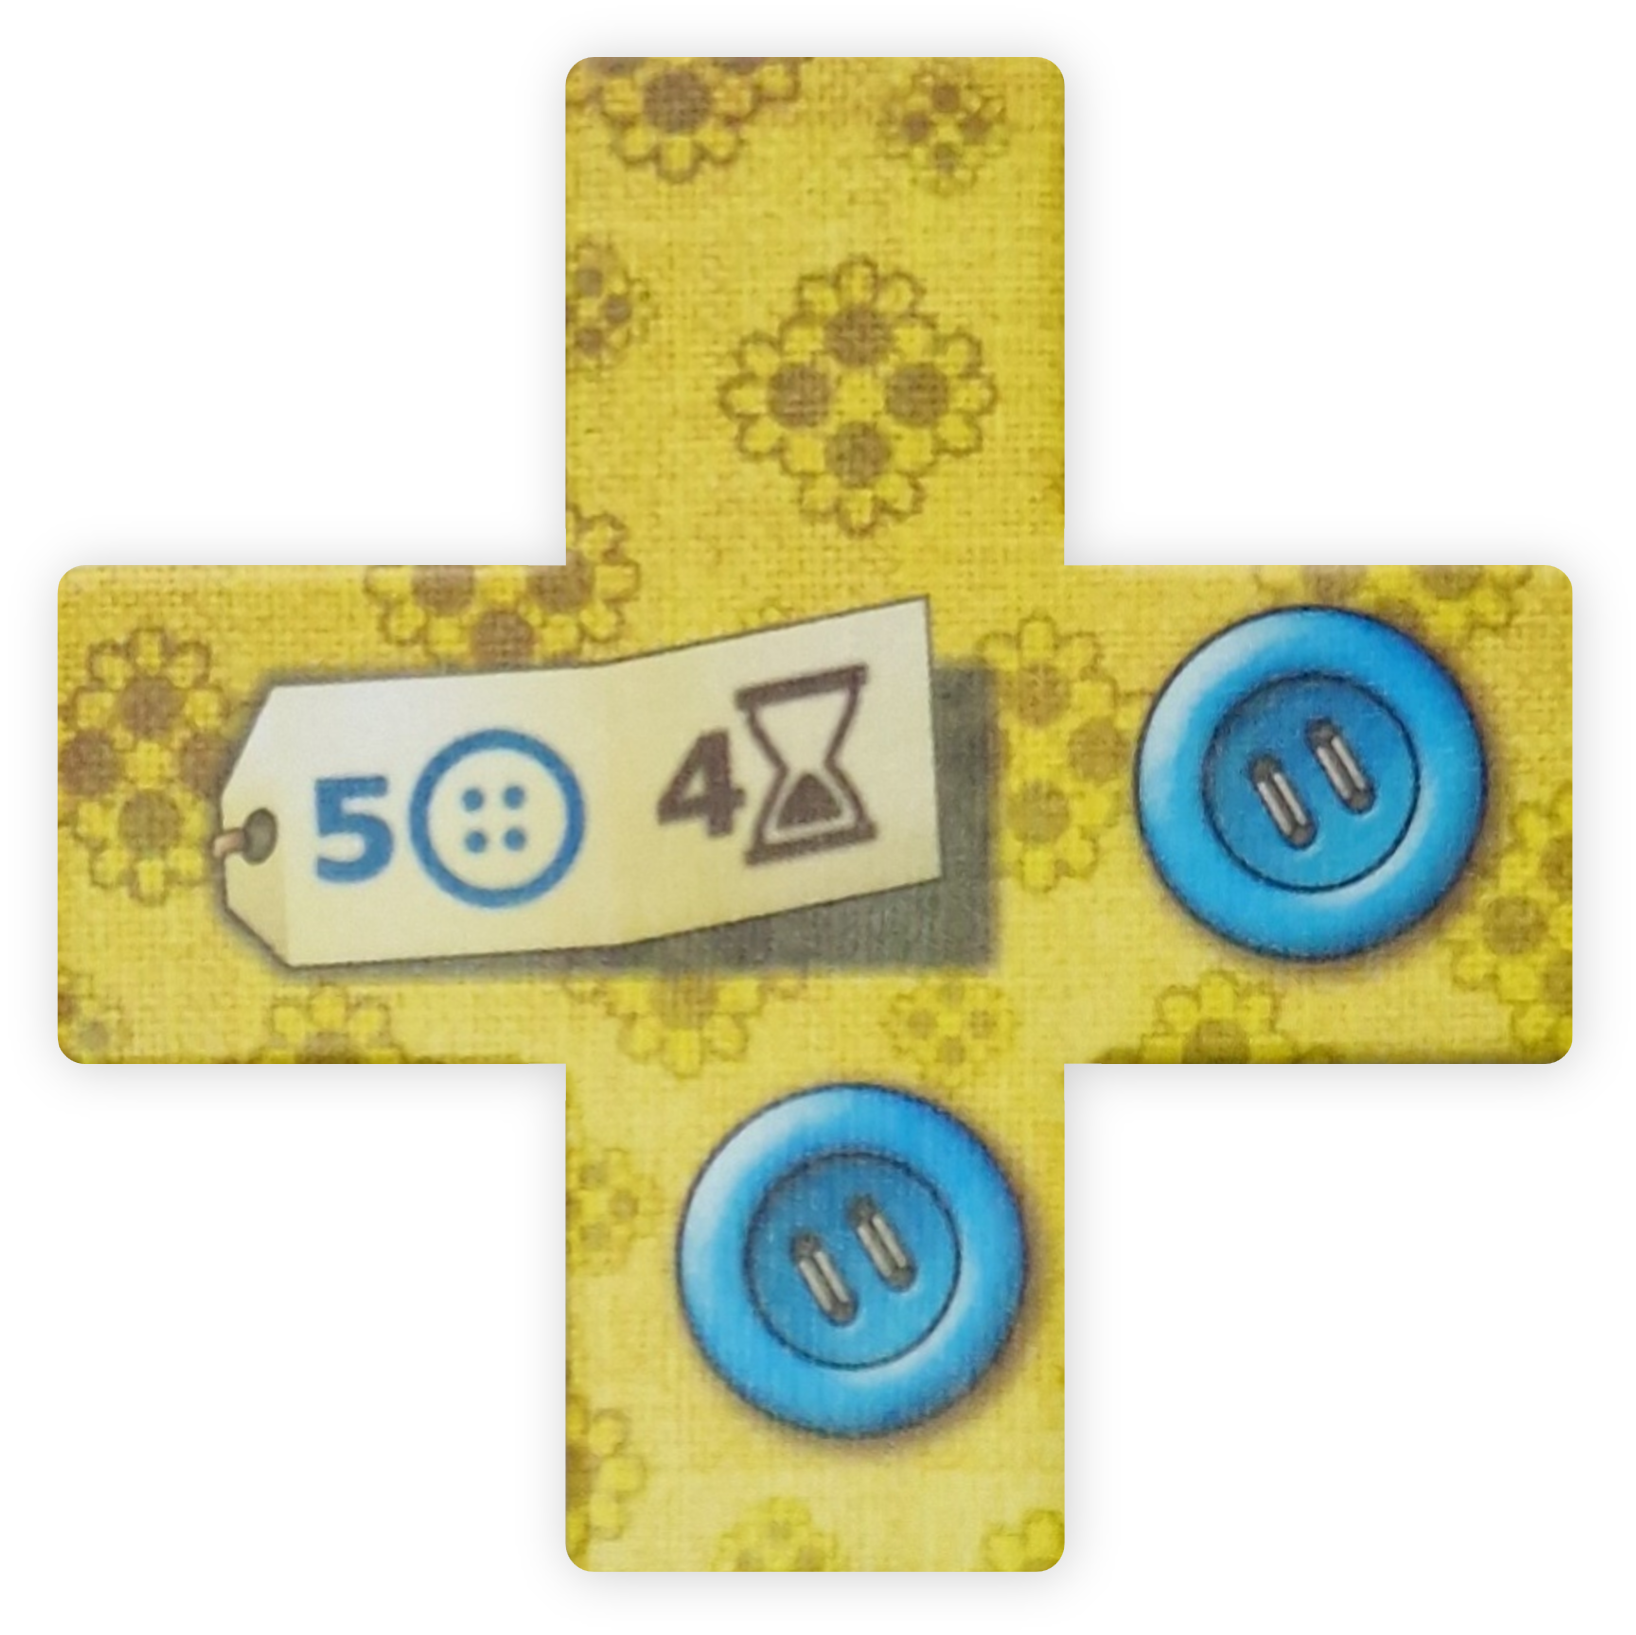
\includegraphics[width=\linewidth]{res/pictures/assets/17-front.png}
    \end{minipage}
    \begin{minipage}{.78\textwidth}
        \centering
        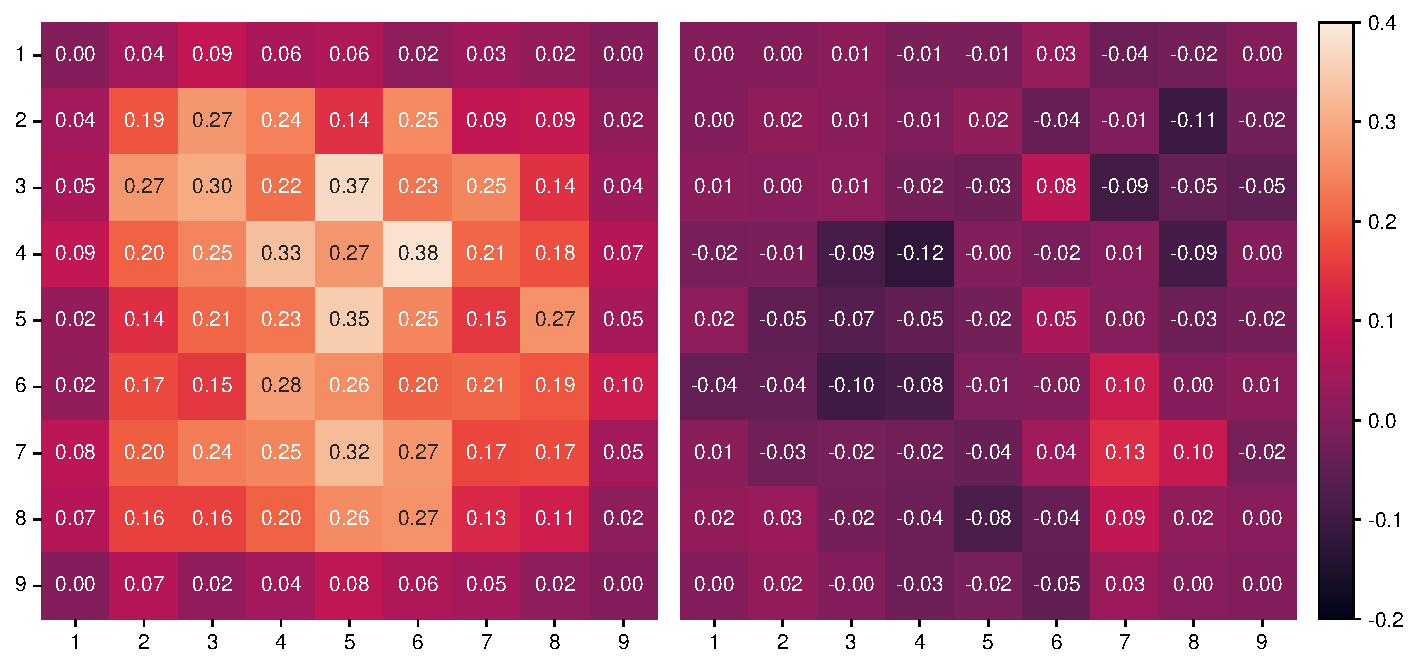
\includegraphics[width=\linewidth]{res/pictures/plots/17-action-ordering.pdf}
    \end{minipage}
    \begin{minipage}{.11\textwidth}
        \hfill
    \end{minipage}
    \vspace*{-0.32cm}
    \captionof{figure}{Heatmap des Flicken 17}
    \label{fig:action-ordering-patch-17}
\end{figure}

\vspace*{-0.36cm}

\begin{figure}[!ht]
    \centering
    \begin{minipage}{.11\textwidth}
        \centering
        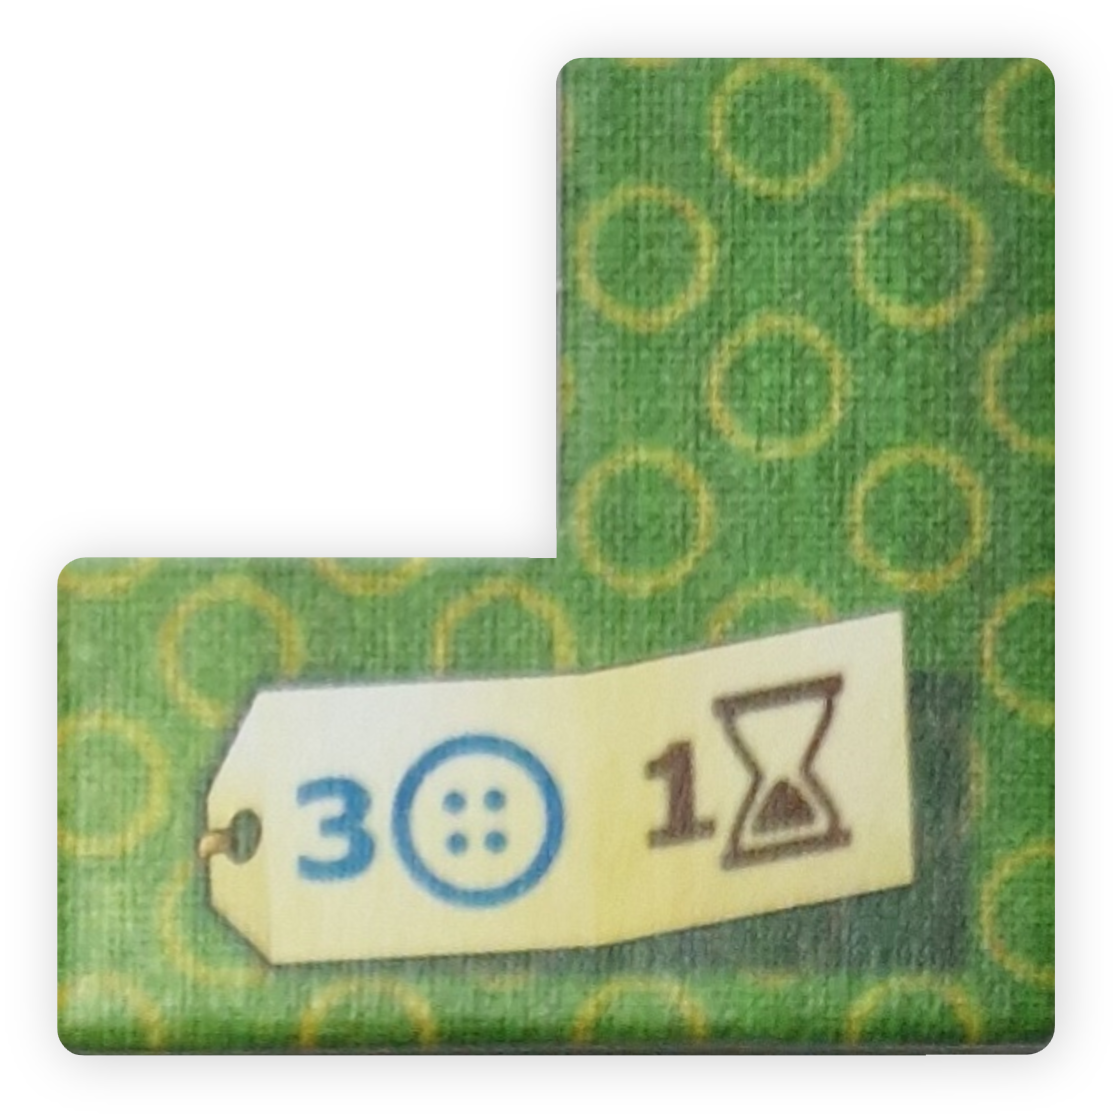
\includegraphics[width=0.667\linewidth]{res/pictures/assets/21-front.png}
    \end{minipage}
    \begin{minipage}{.78\textwidth}
        \centering
        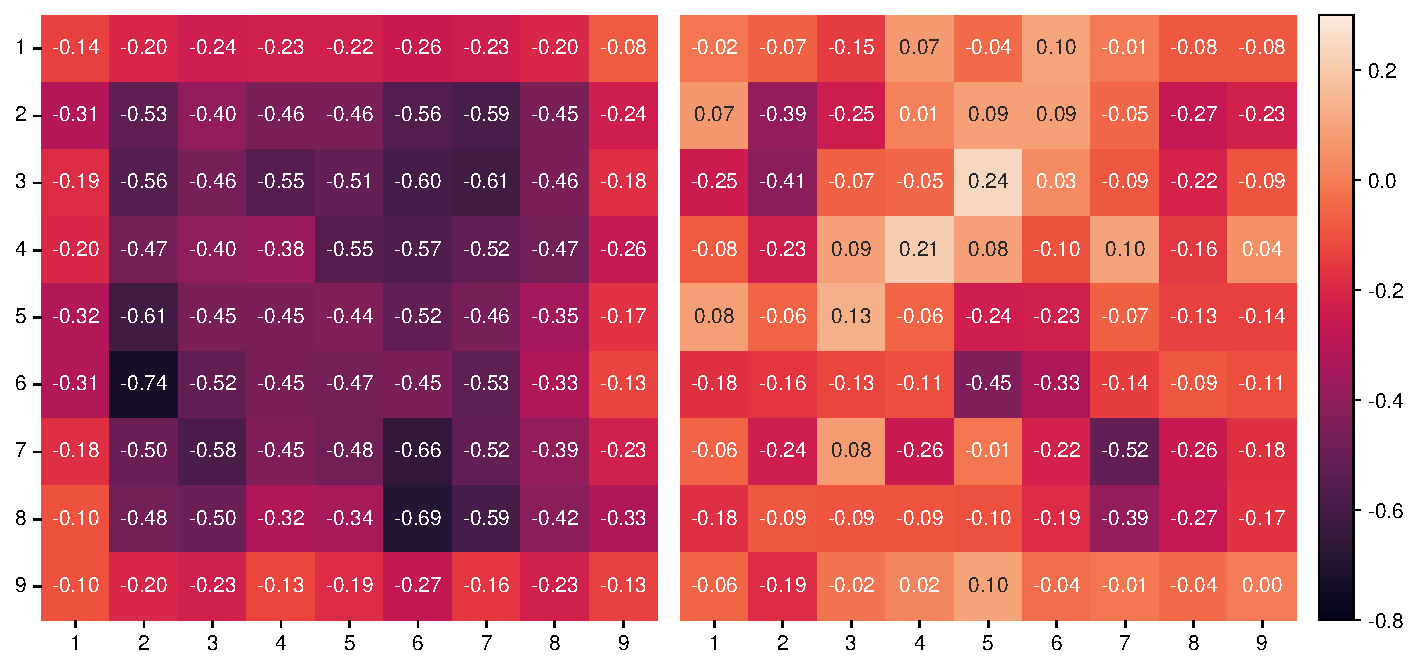
\includegraphics[width=\linewidth]{res/pictures/plots/21-action-ordering.pdf}
    \end{minipage}
    \begin{minipage}{.11\textwidth}
        \hfill
    \end{minipage}
    \vspace*{-0.32cm}
    \captionof{figure}{Heatmap des Flicken 21}
    \label{fig:action-ordering-patch-21}
\end{figure}

\vspace*{-0.14cm}

Der Flicken 17 wird im perfekten Patchwork Spiel zu Beginn des Spiels verwendet, da er sehr viel Knopfeinkommen für einen relativ geringen Preis liefert (siehe \ref{section-loesung-des-optimierungsproblems}). Auch in der Heatmap ist der Flicken deshalb in der Opening-Tabelle mit sehr positiven Werten vertreten, während der Flicken im Endgame durch die hohen Kosten als negativ angesehen wird. Auch die Positionen auf dem Ablageplan stimmen mit der menschlichen Position überein. Flicken 17 ist durch seine kantige Form besser in der Mitte unterzubringen als am Rand des Ablageplans.

Den Erwartungen nach sollte Flicken 21 durch das nicht vorhandene Knopfeinkommen generell weniger wert sein als Flicken 17. Diese Annahme wird auch durch die Heatmap widergespiegelt. Auch, dass die Positionen an den Rändern erwartungsgemäß bei Flicken 21 besser bewertet werden, wird in der Heatmap deutlich. Vor allem verbessert sich die Bewertung von Flicken 21 im späterem Spiel, da dort das Füllen des Ablageplans deutlich relevanter ist als ein nicht existierendes Knopfeinkommen.

Generell sie die Werte der Aktionen nicht perfekt. So müssten die Werte symmetrisch über den Ablageplan verteilt sein, da jeder Spielverlauf auch einfach in einer gedrehten bzw. gespiegelten Form existiert. Dies ist jedoch, wie zu erkennen, nicht der Fall. Weiterhin sind die in Heatmap \ref{fig:action-ordering-special-patch} dargestellten Werte der Spezialflicken zwar wie zu erwarten generell positiv, wirken aber noch sehr zufällig verteilt.

\begin{figure}[!ht]
    \centering
    \begin{minipage}{.78\textwidth}
        \centering
        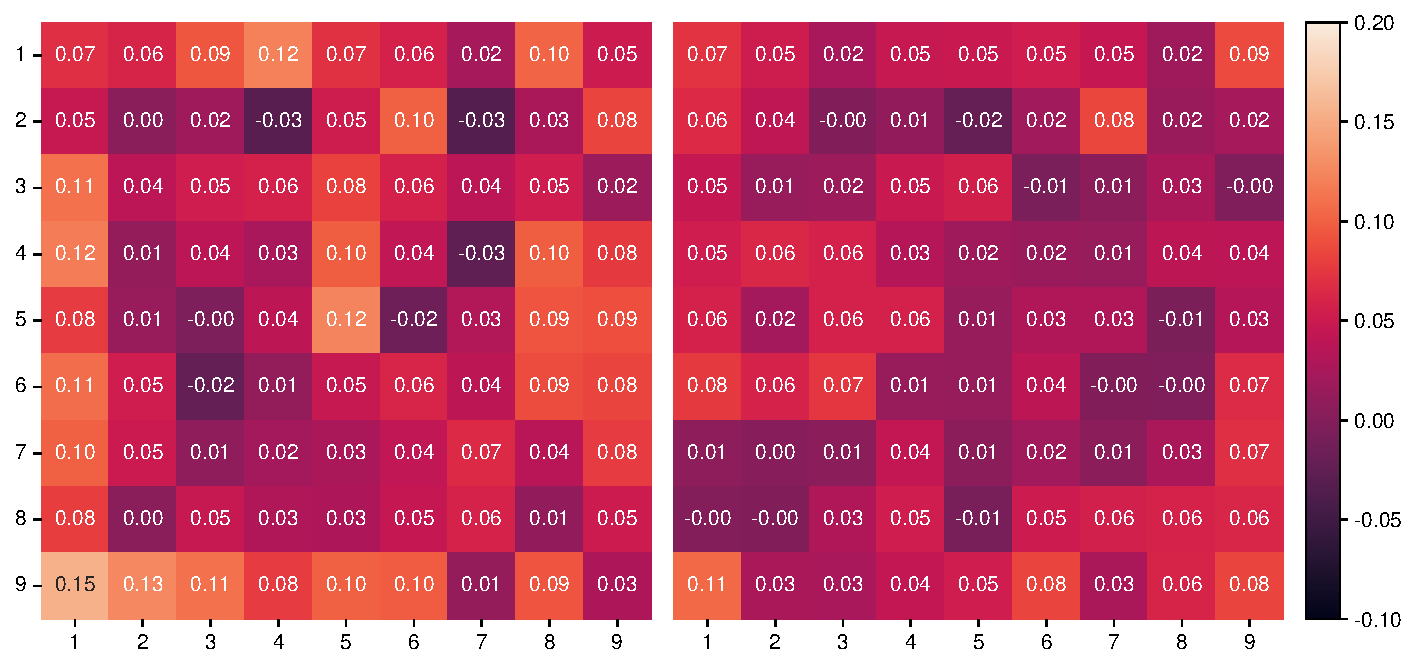
\includegraphics[width=\linewidth]{res/pictures/plots/special-action-ordering.pdf}
    \end{minipage}
    \captionof{figure}{Heatmap des Spezialflicken}
    \label{fig:action-ordering-special-patch}
\end{figure}

\subsection{Transpositionstabelle und Zobrist Hashing}

Für die \ac{PVS} Suche müssen die \ac{PV} Aktionen für jeden Spielzustand gespeichert werden. Nur so kann in der nächsten Iteration diese wieder als erstes durchsucht werden. Weiterhin ist es sinnvoll alle bereits evaluierten Zustände während der Suche zwischenzuspeichern, sodass falls dieser Zustand in einem anderem Teilbaum erneut auftritt, einfach der Wert zurückgegeben werden kann, anstatt erneut den gesamten Teilbaum zu evaluieren. Die Transpositionstabelle dient als Lösung für beide diese Anwendungsfälle.

Die in Patchwork verwendete Transpositionstabelle besteht aus 2 Feldern. Zuerst wird das Alter der Transpositionstabelle gespeichert. Dieses wird im jedem \hyperref[text:ply]{\emph{Ply}} inkrementiert, sodass alte Einträge der Tabelle erkannt und ignoriert werden können. Weiterhin gibt es eine $250 \acsp{MiB}$ große Liste an Tabelleneinträgen. Um jeden Spielzustand einen Eintrag innerhalb der Liste zuzuordnen, muss eine Hashfunktion verwendet. Hierzu wird typischerweise ein \labeltext{\emph{Zobrist Hash}}{text:zobrist-hash} verwendet. Existiert eine Reihe an Elementen, wobei jedes Element nur endliche Menge an Zuständen annehmen kann, so kann jedem Element eine gleichverteilte Zufallszahl zugeordnet werden. Ein \hyperref[text:zobrist-hash]{\emph{Zobrist Hash}} dieser Elemente wird gebildet, indem alle Elemente mittels \ac{XOR} kombiniert werden. \cite[S. 3]{1990.ZobristHash}. Der Vorteil bei der Verwendung von \hyperref[text:zobrist-hash]{\emph{Zobrist Hashes}}  liegt in der schnellen Laufzeitperformance, da nur Indexzugriffe und \ac{XOR}-Bitoperationen verwendet werden.

\vspace*{-0.09cm}

\begin{figure}[!ht]
    \centering
    \includegraphics[width=\textwidth]{res/pictures/zobrist-hash.pdf}
    \vspace*{-0.35cm}
    \caption{Zobrist Hash}
    \label{fig:zobrist-hash}
\end{figure}

\vspace*{-0.2cm}

Der \hyperref[text:zobrist-hash]{\emph{Zobrist Hash}} in Patchwork setzt sich dabei aus den in Abbildung \ref{fig:zobrist-hash} gezeigten Bestandteilen zusammen. Da für alle diese Bestandteile aus dem Kapitel »\nameref{section:spieltheoretische-analyse}« Ober- und Untergrenzen bekannt sind, kann einfach im Voraus ein Array der benötigten Länge mit zufälligen Zahlen erstellt werden. Für den \hyperref[text:zobrist-hash]{\emph{Zobrist Hash}} wird dann einfach mit dem Wert aus dem Spielzustand, \zB das aktuelle Knopfeinkommen, dieses Array indexiert. Gleichermaßen werden alle auf dem Ablageplan gefüllten Felder und die verfügbaren Flicken, mithilfe ihrer \ac{ID} und Distanz zur Spielfigur, sowie alle anderen Bestandteile indexiert und mit in den \hyperref[text:zobrist-hash]{\emph{Zobrist Hash}} mitaufgenommen.

\begin{table}[H]
    \centering
    \begin{tabular}{|c|l|}
        \hline
        Eintrag & Erläuterung                                                                                                      \\ \hline
        Key     & \ac{u64} mit \hyperref[text:zobrist-hash]{\emph{Zobrist Hash}} des Spielzustandes \emph{\acs{XOR}} das Data Feld \\ \hline
        Data    & Die Daten des Eintrags, codiert als ein \ac{u64} von \acs{MSB} nach \ac{LSB} mit:                                \\
                & \tabitem Evaluation (37 Bits): Die Evaluation des Spielzustandes                                                 \\
                & \tabitem Beste Aktion (17 Bits): Die beste Aktion ausgehend vom Spielzustand                                     \\
                & \tabitem Suchtiefe (8 Bits): Die Suchtiefe, bei der der Eintrag eingefügt wurde                                  \\
                & \tabitem Typ der Evaluation (2 Bits): untere Grenze, obere Grenze oder exakt                                     \\ \hline
        Age     & Das Alter des Eintrags.                                                                                          \\ \hline
    \end{tabular}
    \vspace{3pt}
    \caption{Transpositionstabelleneintrag}
    \label{tabelle:transposition-table-entry}
\end{table}

\vspace*{-0.2cm}

Ein Eintrag der Transpositionstabelle ist in Tabelle \ref{tabelle:transposition-table-entry} darstellt. Zuerst wird der Schlüssel (Key) des Spielzustandes gespeichert, um mögliche Hashkollisionen zu erkennen, dann folgen alle relevanten Daten und zuletzt noch das Alter der Transpositionstabelle zum Zeitpunkt des Einfügens, um alte Einträge zu erkennen und zu ignorieren. Die Daten sind dabei in einem besonderen Format gespeichert. Zuerst wird nicht der tatsächliche \hyperref[text:zobrist-hash]{\emph{Zobrist Hash}} als Key, sondern eine \ac{XOR}-Kombination mit den Daten als Schlüssel gespeichert. Weiterhin sind alle Daten in einen \ac{u64} codiert, anstatt diese in einzelnen Feldern zu speichern. All diese Modifikationen dienen dazu, Lockless Hashing zu unterstützen. Die \ac{PVS} Suche soll auch parallel Ablaufen können. Dazu muss die Transpositionstabelle über mehrere Threads geteilt werden. Die geteilte Transpositionstabelle sollte dabei möglichst ohne Locks auskommen, da das häufige Sperren und Freigeben einzelner Einträge ein Performanceoverhead ist.

\begin{lstlisting}[
    label={code:lockless-hashing},
    caption={Einfügen und Lookup bei Lockless Hashing},
    captionpos=b,
    language=Rust,
    escapeinside={<*}{*>},
    numbers=none]
index = zobrist_hash % TABLE_SIZE;

// Einfügen
tt_table[index].<*key*>  = zobrist_hash ^ data;
tt_table[index].data = data;

// Lookup
if (tt_table[index].<*key*> ^ tt_table[index].data == zobrist_hash) {
   // Eintrag gefunden
}
\end{lstlisting}

Lockless Hashing umgeht das Problem von Synchronisation, indem ein Eintrag wie in Quellcode \ref{code:lockless-hashing} eingefügt wird. So kann bei der Lookup-Operation einfach der Key mit dem Data Feld durch ein \ac{XOR} zurück in den \hyperref[text:zobrist-hash]{\emph{Zobrist Hash}} umgewandelt werden. Dadurch, dass in der Lookup-Operation beide Felder verwendet werden, kann so sichergestellt werden, dass Key und Data auch tatsächlich übereinstimmen. Sollte ein anderer Thread gleichzeitig auch nur eines der Felder ändern, so würde die Überprüfung fehlschlagen. Aus diesem Grund können mehrere Threads gleichzeitig den Eintrag lesen und schreiben, ohne dass ein korrupter Zustand aus der Transpositionstabelle ausgelesen werden kann. \cite{2002.LocklessTT}

Das Datenfeld beinhaltet die Evaluation des Spielzustandes, sodass diese in einem anderem Teilbaum wiederverwendet werden kann. Weiterhin wird die beste von diesem Zustand ausgehende Aktion, also die \ac{PV}-Aktion gespeichert. Falls diese nicht bekannt ist, werden die Bits der \emph{Null}-ActionId gespeichert. Die Suchtiefe ist wie das Alter eines Eintrags für Lookup und Ersetzung von Einträgen relevant. Weiterhin wird ein EvaluationTyp gespeichert, welcher einer von drei möglichen Zuständen annehmen kann:

\begin{itemize}
    \item Exakt: Der gespeicherte Spielzustand ist ein \hyperref[text:pv-node]{\acs{PV}-Knoten} und die Evaluation ist somit exakt.
    \item Untere Grenze / Fail-High: Der Knoten ist ein \hyperref[text:cut-node]{Cut-Knoten} und somit ist die gespeicherte Evaluation nur eine untere Grenze für den tatsächlichen Wert des Spielzustands.
    \item Obere Grenze / Fail-Low: Der Knoten ist ein \hyperref[text:all-node]{All-Knoten}. Die Evaluation ist somit nur eine untere Grenze und der tatsächliche Wert kann noch niedriger sein.
\end{itemize}

Für das Einfügen neuer Einträge in die Transpositionstabelle müssen die in Pseudocode \ref{algo:transposition-table-overwrite} dargestellte Bedingungen erfüllt sein. So können leere Einträge oder Einträge aus einem vorherigen \hyperref[text:ply]{\emph{Ply}} immer überschrieben werden. Weiterhin werden alte Einträge überschrieben, falls der neu einzufügende Eintrag für die Evaluation tiefer gesucht hat als der alte Eintrag. Falls also ein bestehender Eintrag existiert, welcher nach der Spielposition noch 3 weitere Ebenen für die Evaluation gesucht hat, wird dieser durch einen neuen Eintrag mit Suchtiefe 4 oder mehr überschrieben. Weiterhin werden Einträge, die nur eine obere oder untere Grenze besitzen durch exakte Evaluationen ausgetauscht.

\pagebreak

\refstepcounter{lstlisting}
\addcontentsline{lol}{lstlisting}{\protect\numberline{\thelstlisting}Pseudocode: Aspiration Windows}

\begin{algorithm}[!ht]
    \caption[Pseudocode: Transpositionstabelle Überschreiben]{Pseudocode: Logik zum Überschreiben von Transpositionstabelleneinträgen}
    \label{algo:transposition-table-overwrite}

    \begin{algorithmic}[1]
        \State \textbf{if} entry.key == 0 \textbf{then}
        \State \hspace*{\algorithmicindent} \Return \emph{Überschreiben} \Comment{Eintrag ist leer}
        \State \textbf{if} entry.age < current\_age \textbf{then}
        \State \hspace*{\algorithmicindent} \Return \emph{Überschreiben} \Comment{Alte Einträge überschreiben}
        \State \textbf{if} entry.data.depth <= new\_depth \textbf{then}
        \State \hspace*{\algorithmicindent} \Return \emph{Überschreiben} \Comment{Einträge mit geringerer Tiefe überschreiben}
        \State \textbf{if} entry.data.depth == new\_depth
        \State \hskip1em \textbf{and} entry.age == current\_age
        \State \hskip1em \textbf{and} entry.data.evaluation\_type != EvaluationType::Exact
        \State \hskip1em \textbf{and} new\_evaluation\_type == EvaluationTyp::Exact \textbf{then}
        \State \hspace*{\algorithmicindent} \Return \emph{Überschreiben} \Comment{Nicht \acs{PV} Einträge überschreiben}
        \State \Return \emph{Nicht Überschreiben}
    \end{algorithmic}
\end{algorithm}

Um den in Abschnitt \ref{subsection:zustandsraum-komplexitaet} aufgezeigten großen Zustandsraum wenigstens teilweise entgegenwirken, wird das Einfügen eines Eintrags noch erweitert. Wenn eine Spielposition erreichbar ist, so ist die gleiche Spielposition mit gedrehten und gespiegelten Ablageplänen beider Spieler ebenso erreichbar und besitzt die gleiche Evaluation. Aus diesem Grund werden all diese symmetrischen Spielpositionen gleichzeitig mit dem originalen Eintrag in die Transpositionstabelle eingefügt.

Um einen Eintrag in der Transpositionstabelle nachzuschauen (Quellcode \ref{code:probe-hash-entry}), muss einfach mit der zuvor vorgestellten Routine überprüft werden, ob der Transpositionstabelleneintrag mit dem Spielstand übereinstimmt. Ist dies der Fall, muss die Suchtiefe des Eintrags größer gleich der noch zu durchsuchenden Tiefe sein. Es macht beispielsweise keinen Sinn einen Transposition Eintrag zu verwenden, der nur noch eine Ebene weitergesucht hat, wenn die eigene Suchfunktion noch mindestens 2 Ebenen tiefer suchen muss. Weiterhin muss beim Lookup auch der EvaluationTyp beachtet werden. Ist der EvaluationTyp ein exakter Wert, kann dieser eingeschränkt auf das $\alpha$-$\beta$-Fenster zurückgegeben werden. Ist nur eine obere Grenze für die Evaluation gespeichert, kann diese nur zurückgegeben werden, wenn sich diese obere Grenze auch unterhalb des $\alpha$-$\beta$-Fensters, also unterhalb von $\alpha$ befindet. Analog verhält es sich mit einer unteren Grenze. Soll nur die \ac{PV}-Aktion aus der Transpositionstabelle ausgelesen werden, sind alle Nebenbedingungen egal. Jedoch kann es dabei vorkommen, dass auch die invalide \emph{Null}-Aktion zurückgegeben wird, da die beste Aktion nicht bekannt ist.

\pagebreak

\lstinputlisting[
    label={code:probe-hash-entry},
    caption={Lookup in der Transpositionstabelle},
    captionpos=b,
    language=Rust,
    firstline=0,
]{res/code/probe-hash-entry.rs}

\pagebreak

\subsection{Aspiration Windows}

Eine mögliche Verbesserung der iterativen Tiefensuche liegt in der Verwendung von Aspiration Windows. Bei der einfachen Implementierung der Tiefensuche ist der initiale Aufruf der \ac{PVS}-Suche immer mit $\alpha = -\infty$ und $\beta = \infty$. Bei Aspiration Windows wird diese Annahme insofern aufgelockert, indem davon ausgegangen wird, dass sich der Wert der nächsten Suchiteration nicht viel von dem Wert der vorherigen Suche unterscheidet. Deshalb wird statt dem gesamten Bereich nur ein Fenster (Aspiration Window) der Größe $\Delta$ um den vorherigen Suchwert erkundet. \cite{2003.AspirationWindows}

Da das initiale Fenster deutlich schmaler ist, können während der Suche im Normalfall mehr $\beta$-Cutoffs erreicht werden, was somit gleichzeitig einer kürzeren Suche entspricht. In den meisten Fällen gibt die Suche mit dem Aspiration Window auch wieder einen Wert innerhalb des Fensters von $\alpha$ und $\beta$ zurück. Ist dies nicht der Fall, muss die Suche zwingend erneut mit einem breiterem Aspiration Window wiederholt werden, was ein Nachteil bei der Verwendung ist.

\refstepcounter{lstlisting}
\addcontentsline{lol}{lstlisting}{\protect\numberline{\thelstlisting}Pseudocode: Aspiration Windows}

\begin{algorithm}[!ht]
    \caption{Pseudocode: Iterative Tiefensuche mit Aspiration Windows}
    \label{algo:aspiration-window}
    \begin{algorithmic}[1]
        \Function{search}{$game$}
        \State $\alpha \gets $ Starting-$\alpha$,\ \ $\beta \gets $ Starting-$\beta$,\ \ $\Delta \gets $ Starting-$\Delta$
        \For{$depth \coloneq 0$ bis Maximaltiefe}
        \State $value \gets \Call{principal\_variation\_search}{$\alpha$,\,$game$,\,$\beta$}$
        \If{Suchzeit vorbei}
        \State \textbf{break}
        \ElsIf{$value \le \alpha$} \Comment{Aspriation Window Fail-Low}
        \State $\alpha = value - \Delta$
        \State $\beta = (\alpha + \beta) / 2$ \Comment{$\beta$ in die Mitte des Fenster}
        \State $\Delta = \sfrac{4}{3}\cdot \Delta$
        \State \textbf{continue}
        \ElsIf{$value \ge \beta$} \Comment{Aspriation Window Fail-High}
        \State $\beta = value + \Delta$
        \State $\Delta = \sfrac{4}{3}\cdot \Delta$
        \State \textbf{continue}
        \EndIf
        \State $\Delta = $ \Call{new\_delta}{$value$,\, Starting-$\Delta$}
        \State $\alpha = value - \Delta$
        \State $\beta = value + \Delta$
        \EndFor
        \EndFunction
    \end{algorithmic}
\end{algorithm}

Wird ein Wert unterhalb von $\alpha$ zurückgegeben, handelt es sich um einen \emph{Fail-Low}, ist der Wert oberhalb von $\beta$, ist es ein \emph{Fail-High} Fall. Um im solch einen Failing-Fall möglichst effizient zu agieren, wird das Aspiration Window oftmals mit einem exponentiellen Backoff breiter gemacht, bis der Wert der Suche innerhalb des Fensters liegt. Die im Pseudocode \ref{algo:aspiration-window} verwendeten Werte für die Anpassung von $\alpha$, $\beta$ und $\Delta$ entsprechen dabei den Werten, welche in Stockfish verwendet werden, was eine der besten Schach-Computerspielengines ist \cite{2024.StockfishBackoff} \cite{2024.Stockfish}. Aus diesem Grund verwendet der \ac{PVS}-Spieler den gleichen exponentiellen Backoff. Bei einer einfachen Minimax-Suche lässt sich in einem Fail-Fall die Fenstergrenze, welche nicht fehlgeschlagen ist, immer auf die andere Grenze setzen. Kommt es also zu einem Fail-High bei der Suche mit Aspiration Window $\left[\alpha, \beta\right]$, so könnte die nächste Suche mit $\left[\beta, \beta + \Delta\right]$ stattfinden. Bei der Suche des \ac{PVS}-Spielers ist dies aufgrund von Suchinstabilität nicht der Fall. Suchinstabilität heißt, dass eine wiederholte Suche eines Spielzustands nicht immer die gleiche Evaluation zurückgeben muss \cite{2003.SearchInstability}. Diese Suchinstabilität kann bereits durch die Verwendung der gespeicherten Evaluationen aus der Transpositionstabelle entstehen \cite{2003.SearchInstability}. Im Falle der Aspiration Windows bedeutet dies, dass eine Suche, die vorher mit Fail-High abgebrochen wurde, in der darauffolgenden Suche einen Fail-Low erzeugen kann. Deshalb wird der Wert von $\beta$ im Pseudocode zum Beispiel nur in die Mitte des Fensters verschoben.

\subsection{Suchselektivität}

Shannon führt in seinem Werk \emph{\enquote{Programming a Computer for Playing Chess}} eine Klassifizierung der Suchmethoden in einem Spielbaum ein, die zwei Haupttypen umfasst: \textbf{Typ-A} ist eine vollständige Brute-Force-Suche durch den gesamten Baum bis zu einer gewissen Tiefe \cite[S. 8]{1950.ChessShannon}. Bei der \textbf{Typ-B} werden die Äste des Spielbaums so selektiv ausgewählt, dass interessante Teilbäume tiefer durchsucht werden und uninteressante Teilbäume nur reduziert oder gar nicht durchsucht werden.

Im Bereich der Sucherweiterungen werden in Schach normalerweise Aktionen wie das Schlagen von Schachfiguren oder Schachsetzen des Königs berücksichtigt \cite[S. 14]{1950.ChessShannon}\cite{2023.StockfishTerminology}\cite{2002.SearchExtensions}. Während solche Aktionen in Patchwork nicht existieren, gibt es zwei Ereignisse, die für einen Spieler besonders interessant sind: Das Erhalten des $7\times 7$ Sonderplättchens sowie das Legen eines Spezialflicken. Bei beiden Aktionen wird die Suche deshalb um eine Tiefenebene erhöht (Anhang \ref{code:pvs-search-extension}). Im Fall der Null-Fenster-Suche werden keine Sucherweiterungen angewendet.

\vspace*{-5cm}

\pagebreak

Für Patchwork sind Suchreduktionen im Bereich der Typ-B-Suche jedoch von größerer Bedeutung. Um bei Spielzuständen, die viele Aktionen erlauben und somit einen hohen Verzweigungsfaktor haben, den Suchaufwand möglichst minimal zu halten, sollte ein großer Teil der Aktionen nur reduziert durchsucht oder ganz weggelassen werden. Im \ac{PVS}-Spieler kommen hierzu zwei Konzepte zum Einsatz: \ac{LMR} und \ac{LMP}.

Bei einer Suche mit einigermaßen guter Zugreihenfolge tritt ein \hyperref[text:beta-cutoff]{\emph{Beta-Cutoff}} wenn überhaupt normalerweise am ersten \acs{PV}-Knoten auf \cite{2007.LMR}. Deswegen werden bei \ac{LMR} nur die ersten Aktionen mit der vollen Tiefe durchsucht und alle weiteren Aktionen werden, insofern nichts Interessantes passiert, mit einer reduzierten Tiefe durchsucht. Als Nachteil muss bei einem zu guten Ergebnis über $\alpha$ der Teilbaum mit voller Tiefe erneut durchsucht werden \cite{2007.LMR}. Im \ac{PVS}-Spieler wird die Suche bei allen nicht \ac{PV}-Aktionen ab einer gewissen Tiefe auf ein Drittel der originalen Tiefe reduziert. Vorher wird die Suche immer um eine Ebene reduziert.

Bei \ac{LMP} wird ein noch drastischerer Ansatz verfolgt, indem bestimmte Teilbäume gar nicht mehr anstatt nur reduziert durchsucht werden \cite{2023.StockfishTerminology}. Dabei handelt es sich um einen Tradeoff zwischen Suchgenauigkeit bzw. -stabilität und Zeit. Je mehr Aktionen \emph{geprunt}, also weggelassen werden, desto tiefer kommt die Suche. Gleichzeitig könnten aber so Teilbäume übersehen werden, welche einen besseren Spielverlauf beinhalten. Um die sehr große Anzahl an Aktionen, die bei einem Spielzustand auftreten können (1345) zu reduzieren, werden sehr viele Aktionen im \ac{PVS}-Spieler geprunt. Während in der ersten Ebene immer alle Aktionen betrachtet werden, wird in den späteren Tiefen immer nur sichergestellt, dass mindestens 3 Platzierungsmöglichkeiten für jeden Flicken überprüft werden. Die Auswahl dieser Aktionen basiert dabei auf der Bewertung der Aktionen-Anordnung. Die spezifischen Pruning-Werte wurden ermittelt, indem verschiedene Konfigurationen für die Starttiefe und die Anzahl an Platzierungsmöglichkeiten pro Flicken mit dem klassischen Alpha-Beta-Minimax-Algorithmus (wie in \ref{algo:minimax-alpha-beta}) gegeneinander spielten. Dabei wurden die besten Werte für den \ac{PVS}-Spieler übernommen.

\pagebreak

\subsection{Lazy-SMP}

Der bisher beschriebene \ac{PVS}-Spieler läuft Single-Threaded ab. Da heutige Computer mehrere Kerne besitzen, sollten diese auch verwendet werden. Für Minimax sowie davon abgeleitete Algorithmen existiert dazu eine einfache, aber gleichzeitig so effektive Parallelisierungsmöglichkeit, dass selbst die besten Schachengines diese verwenden \cite{2016.Stockfish7} \cite[S. 52]{2016.ParallelChessEngine}.

Bei Lazy \ac{SMP}, werden $n$ parallele unabhängige Suchen gleichzeitig gestartet, welche sich nur die Transpositionstabelle teilen. Dadurch, dass alle bereits durchsuchten Spielzustände in die Transpositionstabelle eingefügt werden, wird sichergestellt, dass Spielzustände, welche zuvor von Threads erkundet wurden, nicht erneut durchsucht werden müssen. Dadurch, dass die Transpositionstabelle bereits Lockless Hashing verwendet, können im Code einfach neue Threads gestartet werden, ohne dass weitere Synchronisationsmechanismen eingebaut werden müssen. Nachdem die Zeit abgelaufen ist, werden alle Threads gestoppt und die \ac{PV} Aktion aus der Transpositionstabelle ausgelesen.

\pagebreak

\section{Ansatz D: Monte Carlo Tree Search}
\label{section:erstellung-ansatz-c}

Der \ac{MCTS} Spieler verwendet zur Suche nach der besten Aktion den \acl{MCTS} Algorithmus. Dabei werden die vier Phasen immer wieder wie in Quellcode \ref{code:mcts-playout} wiederholt, bis eine vorgegebene Endbedingung erreicht ist. Im Regelfall ist diese Endbedingung ein Zeitlimit, kann aber zu Testzwecken auch durch eine Anzahl an Iterationen der vier Phasen angegeben werden. Der \ac{MCTS} Spieler selbst übernimmt keine Suche, sondern erstellt mit dem gegebenen Spielzustand einen neuen Suchbaum. Innerhalb des Suchbaums sind die \ac{MCTS} Phasen implementiert. Der \ac{MCTS} Spieler ruft dann, solange die Endbedingung nicht erreicht ist, immer wieder die \code{playout} Methode im Suchbaum auf. Am Ende wird dann die Aktion ausgewählt, bei der der assoziierte Knoten im Suchbaum am meisten Besuche hat, da dies der Knoten ist, welcher die größte Gewinnwahrscheinlichkeit besitzt \cite[S. 217]{2008.MCTS}.

\lstinputlisting[
    label={code:mcts-playout},
    caption={[Die vier Phasen einer MCTS Iteration]Die vier Phasen einer \acs{MCTS} Iteration},
    captionpos=b,
    language=Rust,
    firstline=0,
]{res/code/mcts-playout.rs}

Die einzelnen Knoten innerhalb des Suchbaums werden durch die in Quellcode \ref{code:mcts-node} dargestellte Struktur \code{Node} modelliert. Jedem Knoten wird neben einer \ac{ID} und dem Spielzustand, den der Knoten repräsentiert auch ein optionaler Elternknoten zugeordnet, der immer vorhanden ist, solange es sich nicht um die Wurzel des Suchbaums handelt. Die Wurzel des Suchbaums entspricht den Ausgangszustand, bei dem der \ac{MCTS} Spieler eine Aktion auswählen soll. In \code{action\_taken} ist die Aktion gespeichert, welche verwendet wurde, um vom dem Spielzustand des Elternknotens in den Spielzustand des Knotens zu gelangen. Weiterhin gibt es eine Liste an Kinderknoten. Diese Liste ist nach dem \ac{MCTS} Algorithmus jedoch zu Beginn leer und füllt sich erst mit der Zeit durch die Expansionsphase. Um zu überwachen, welche Knoten bereits existieren, gibt es noch eine List mit expandierbaren Aktionen. Diese ist zu Beginn mit allen aus dem Spielzustand verfügbaren Aktionen gefüllt. Wird innerhalb der Expansionsphase ein neuer Knoten erstellt, so wird die entsprechende Aktion aus der Liste entfernt. Ist die Liste leer, so ist ein Knoten vollständig expandiert. Zuletzt wird noch eine Reihe von statistischen Kenngrößen gespeichert, die für die Auswahl der Knoten mittels einer \enquote{Tree Policy} innerhalb der Selektionsphase von \ac{MCTS} benötigt werden. Die \emph{neutral} Werte sind dabei immer aus Sicht des ersten Spielers gespeichert, anstatt aus Sicht des Spielers, welcher in dem Spielzustand des Knotens gerade an der Reihe ist.

\lstinputlisting[
    label={code:mcts-node},
    caption={[Knoten im MCTS-Baum]Knoten im \acs{MCTS}-Baum},
    captionpos=b,
    language=Rust,
    firstline=0,
]{res/code/mcts-node.rs}

\pagebreak

Die einzelnen Knoten verweisen dabei mit \emph{NodeIds} aufeinander, anstatt mit direkten Referenzen, um die Rust-Ownership Regeln einzuhalten. In Rust darf ein Objekt nur von einem anderen Objekt \enquote{besitzt} werden. Wird ein Knoten durch seinen Eltern- als auch seine Kindknoten referenziert, so ist dieser eindeutige Besitz nicht mehr geregelt. Aus diesem Grund werden alle Knoten außerhalb des Suchbaums in einem Array gespeichert und mittels der NodeId referenziert.

\subsection{Tree Policy}

In der Selektionsphase einer \ac{MCTS} Iteration muss ausgehend von dem Wurzelknoten immer ein weiterer Knoten ausgewählt werden, bis ein Knoten erreicht wird, bei dem noch nicht jede Aktion einmal ausprobiert wurde oder bei dem es sich um einen Terminalknoten handelt, also einen Knoten wo der assoziierte Spielstand ein Endzustand ist. Für die Selektion wird eine \enquote{Tree Policy} verwendet. Die Tree Policy betrachtet alle Kinderknoten eines Knotens und entscheidet sich für einen der Knoten. Dazu wird im Normalfall jedem Kinderknoten ein Wert zugeordnet und der Knoten mit dem höchsten Wert ausgewählt. Bei dem \ac{MCTS} Spieler stehen dabei 3 mögliche Tree Policies zur Auswahl.

\begingroup
\allowdisplaybreaks
\begin{align}
    \mathbb{UCT}                         & = \frac{w}{n} + c \cdot \sqrt{\frac{\ln N}{n}}                                                                                                                                                                                                                                                                                                                                                                                                                                                                                                                                                                                                                                                                                                                                                                                                                                                                                                                                                                                                                                                                                 \\  \notag
    \intertext{Die erste Tree Policy ist die bereits aus dem \nameref{chapter:grundlagen}-Kapitel bekannte \acf{UCT} Formel. Der Name \ac{UCB} kommt daher, dass diese Formel auch als obere Grenze eines Konfidenzintervalls gesehen werden kann. So wird mit dem exploitativen Teil, der Gewinnrate ($\sfrac{w}{n}$) des Knotens, ein Punktschätzer für den wahren Wert des Knotens erstellt. Da diese Schätzung bei kleinen $n$ jedoch relativ ungenau ist, wird die Unsicherheit bzw. Varianz der Schätzung durch den explorativen Teil, dem Verhältnis aus Anzahl von Besuchen der Eltern- und Kindknoten ($\sqrt{\frac{\ln N}{n}}$), angegeben \cite[S. 36]{2018.ReinforcementLearning}. Durch die Kombination beider Terme ergibt sich somit durch Punktschätzer und Varianz die obere Grenze eines Konfidenzintervalls, bei dem der wahre Wert mit großer Wahrscheinlichkeit unterhalb dieser Grenze liegt. Die \ac{UCT} Formel selektiert nun den Knoten mit der größten oberen Grenze, um dieses Maximum entweder zu bestätigen oder die Schätzung anzupassen.}                                                                                                        \notag \\
    \text{Scored-}\mathbb{UCT}           & = \frac{\sum s_i}{n} + c \cdot |\max S_i - \min_i S_i| \cdot \sqrt{\frac{\ln N}{n}}                                                                                                                                                                                                                                                                                                                                                                                                                                                                                                                                                                                                                                                                                                                                                                                                                                                                                                                                                                                                                                            \\ \notag
    \intertext{Die zweite mögliche Tree Policy erweitert die \ac{UCT} Formel insofern, dass auch das tatsächliche Ergebnis eines Patchwork Spiels in der Entscheidung eine Rolle spielt. Während bei \ac{UCT} einfach nur eine Gewinnrate berechnet wird, verwendet Scored-$\mathbb{UCT}$ die Endergebnisse, indem der Mittelwert dieser als exploitativer Teil berechnet wird ($\sfrac{\sum s_i}{n}$). Da hierbei der exploitative Teil außerhalb von $\left[0,1\right]$ fallen kann, muss auch der explorative Teil entsprechend skaliert werden. Das geschieht dadurch, dass die Differenz zwischen dem höchsten und niedrigsten Gewinn, welcher im Elternknoten im Laufe der Zeit aufgetreten ist, berechnet wird ($|\max S_i - \min_i S_i|$) und zum Skalieren verwendet wird.}                                                                                                       \notag                                                                                                                                                                                                                                                                           \\
    \text{Partially-Scored-}\mathbb{UCT} & = \rho \cdot \text{Scored-}\mathbb{UCT} + (1 - \rho) \cdot \mathbb{UCT}
\end{align}
\endgroup

Die dritte Tree Policy kombiniert die beiden ersten Ansätze, indem eine lineare Interpolation zwischen $\mathbb{UCT}$ und Scored-$\mathbb{UCT}$ bereitgestellt wird. Der Hyperparameter $\rho$ bestimmt dabei zu wie viel Prozent die einzelnen Terme in die Gesamtwertung eingehen sollen. Die Performance der einzelnen Tree Policies wird in Kapitel \ref{chapter:evaluation} verglichen.

\subsection{Evaluator}

Für die Simulationsphase von \ac{MCTS} kann einfach das bereits zuvor vorgestellte Evaluator-Trait verwendet werden. Dies hat den Vorteil, dass verschiedene Rollout-Mechanismen leicht austauschbar und gegeneinander testbar sind. So wird der Standard-Rollout-Mechanismus für die Simulation mit dem Wählen von zufälligen Aktionen und dem anschließenden Backpropagieren von Gewinn oder Verlust bereits durch den Win-Loss-Evaluator bereitgestellt. Genauso gut kann aber durch den Austausch des Win-Loss-Evaluators mit den Score-Evaluator das tatsächliche Endergebnis der zufälligen Spiele miteinbezogen werden.

\subsection{Wiederverwendung des Suchbaums}

Um Kenntnisse aus den vorherigen vorherigem \hyperref[text:ply]{\emph{Plys}} zu verwenden, wird der Suchbaum von dem \ac{MCTS} Spieler nach Möglichkeit wiederverwendet. Dabei besteht die Hoffnung, dass der Wurzelknoten der neuen Suche bereits als ein Knoten im Suchbaum eines vorherigen \hyperref[text:ply]{\emph{Plys}} enthalten ist. Dann könnte dieser Knoten als neuer Wurzelknoten verwendet werden und von dort die Suche gestartet werden. Alle bereits bestehenden Knoten im alten Suchbaum können dann direkt zusammen mit den bereits erworbenen Kenntnissen über die zugrundeliegende Wahrscheinlichkeitsverteilungen für das Gewinnen übernommen werden. Ziel ist es, somit die Anzahl der \ac{MCTS} Iterationen innerhalb eines Zeitraums \enquote{künstlich} zu erhöhen, indem alte Iterationen direkt übernommen werden.

Das Hauptproblem liegt dabei, herauszufinden, welcher Knoten im alten Suchbaum mit dem Wurzelknoten im neuen Suchbaum korrespondiert. Generell kann ein Spieler direkt 2-mal hintereinander dran sein, womit sich der neue Wurzelknoten direkt in der ersten Ebene des alten Suchbaums befindet. Genauso ist es aber möglich, dass nach einem Zug des \ac{MCTS} Spielers erst einmal bis zu 7 Züge des gegnerischen Spielers folgen (siehe \ref{subsection:analyse-maximale-anzahl-aufeinanderfolgender-plys}). In solchen Fällen könnte es sinnvoller sein, die Suche direkt mit einem neuen Suchbaum zu beginnen, anstatt den Suchaufwand im alten Baum zu betreiben. Der Grund dafür ist, dass Zeit mit der Suche verloren geht, welche besser dafür verwendet werden kann, neue \ac{MCTS} Iterationen durchzuführen. Das ist vor allem der Fall, da die Wahrscheinlichkeit, dass in der achten Ebene im alten Suchbaum überhaupt so viele Iterationen und somit ein großer Teilbaum existieren, recht gering ist. Als Kompromiss wird deshalb im \ac{MCTS} der alte Suchbaum immer übergeben und eine Breitensuche entlang diesem Suchbaum nach dem neuen Wurzelknoten wie in Codeausschnitt \ref{code:mcts-node} durchgeführt. Diese Breitensuche wird beendet, sobald der neue Wurzelknoten gefunden ist oder abgebrochen, wenn das erste Mal ein Knoten in der achten Ebene des alten Suchbaums auftritt. Wurde der neue Spielzustand nicht innerhalb der ersten sieben Ebenen gefunden, so existiert er im alten Suchbaum einfach nicht, zum Beispiel da zuvor nicht genügend Iterationen stattgefunden haben, um auch diesen Zustand zu erreichen. Weiterhin wird die Suche nach dem neuem Wurzelknoten auch nach einer gewissen Zeit verfrüht abgebrochen, um nicht zu viel Zeit mit der Suche im alten Suchbaum zu verbringen. Als Zeitlimit wird hierbei 2 \acp{ms} verwendet. In dieser Zeit können im alten Suchbaum mehrere Ebenen durchsucht werden, während gleichzeitig nicht zu viel Zeit für die Suche verloren geht.

\lstinputlisting[
    label={code:mcts-node},
    caption={[Wiederverwendung des MCTS-Suchbaums]Wiederverwendung des \acs{MCTS}-Suchbaums},
    captionpos=b,
    language=Rust,
    firstline=0,
]{res/code/mcts-tree-reuse.rs}

Die Suche nach dem neuen Spielzustand innerhalb des alten Teilbaums ließe sich in Zukunft noch dadurch verbessern, dass einfach alle Aktionen, die seit der letzten Aktion des \ac{MCTS} Spielers passiert sind, gespeichert werden. Diese Aktionenfolge kann dann im alten Suchbaum so lange verfolgt werden bis entweder der passende Spielzustand und somit der Teilbaum gefunden ist oder kein weiterer passender Knoten mehr existiert.

\subsection{Parallelisierung}

Für die Parallelisierung von \ac{MCTS} existieren wie in Abbildung \ref{fig:mcts-parallization} dargestellt 3 verschiedene Varianten.

\vspace*{-0.3cm}
\begin{figure}[!ht]
    \centering
    \includegraphics[width=\textwidth]{res/pictures/mcts-parallization.pdf}
    \vspace*{-0.75cm}
    \caption[Parallelisierungsmöglichkeiten bei MCTS]{Parallelisierungsmöglichkeiten bei \acs{MCTS}}
    \label{fig:mcts-parallization}
\end{figure}
\vspace*{-0.15cm}

Bei der \labeltext{\emph{Leaf Parallelisierung}}{text:leaf-parallelization} finden die \ac{MCTS} Phasen Selektion und Expansion wie normal statt. Nur während der Simulations-Phase werden mehrere Threads gestartet, welche alle verschiedene zufällige Spielverläufe ausgehend von dem ausgewählten Knoten simulieren. So können in der Backpropagation-Phase gleich mehrere Spielausgänge im Baum rückpropagiert werden, sodass für den Zustand direkt eine etwas genauere Schätzung bei einer einzigen \ac{MCTS} Phase besteht. Nachteil hierbei ist, dass immer gewartet werden muss, bis alle Threads ihren simulierten Spielverlauf fertig gestellt haben und sonst keine Parallelisierung stattfindet. Somit schafft diese Parallelisierungsart insgesamt weniger vollständige \ac{MCTS} Iterationen als die Single-Threaded-Variante. \cite[S. 204]{2016.HybridMCTS}

\vspace*{-5cm}

\pagebreak

Die \labeltext{\emph{Root Parallelisierung}}{text:root-parallelization} ist ebenso wie die \hyperref[text:leaf-parallelization]{\emph{Leaf Parallelisierung}} leicht umzusetzen. Anstatt dass nur ein einziger \ac{MCTS}-Suchbaum existiert, wird einfach für jeden Thread ein neuer Suchbaum erstellt. Während der Suchzeit führen die Threads dann auf ihrem Suchbaum eine einfache Singe-Threaded-\ac{MCTS}-Suche durch. Am Ende werden einfach die Knoten aller Bäume aus der ersten Ebene kombiniert. Dies kann einfach über die Aktion geschehen, welche verwendet wurde, um vom Wurzelknoten zu dem Knoten in der ersten Ebene zu kommen. Die ausgewählte Aktion des Spielers ist die Knotenkombination, welche insgesamt am meisten Besuche durch alle Threads besitzt. \cite[S. 63]{2008.ParallelMCTS}

Die dritte Parallelisierungsart, die \labeltext{\emph{Tree Parallelisierung}}{text:tree-parallelization} sorgt für eine gemeinsame Suche von mehreren Threads innerhalb eines Baums. Dazu werden am jedem Knoten Sperren, wie beispielsweise Mutexe, verwendet. Möchte ein Thread die Werte des Knotens lesen oder modifizieren wird einfach eine Lese- bzw. Schreibsperre gesetzt. In diesem Zeitraum können keine anderen Threads auf diesen Knoten zugreifen. Da alle Threads Knoten nach der gleichen Tree Policy selektieren, würde diese Implementierung dazu führen, dass alle Threads immer die gleichen Knoten im Baum selektieren und somit auf einem sehr ähnlichen Pfad durch den Baum traversieren. Dies führt dazu, dass die Threads sich dauernd durch Sperren gegenseitig zum Warten zwingen, was den Sinn von Parallelisierung entgegenwirkt. Aus diesem Grund wird noch das Konzept eines \emph{Virtual Loss} eingeführt. Sobald ein Thread einen Knoten selektiert hat, wird der \emph{Virtual Loss} inkrementiert und erst wieder dekrementiert, wenn der Thread mit der Backpropagation-Phase fertig ist und eine neue \ac{MCTS}-Iteration anfängt. Der \emph{Virtual Loss} verhält sich dabei wie normale Niederlagen durch die Simulationsphase. Da bei der Selektion Knoten bevorzugt werden, bei denen die Gewinnrate möglichst hoch ist, bevorzugen die anderen Threads dann einen anderen Pfad durch den Suchbaum und es kommt zu weniger Sperren. \cite[S. 64]{2008.ParallelMCTS}

Für den \ac{MCTS} Spieler wurden die Parallelisierungsarten \hyperref[text:leaf-parallelization]{\emph{Leaf Parallelisierung}} und \hyperref[text:root-parallelization]{\emph{Root Parallelisierung}} umgesetzt. Diese lassen sich leicht in den bereits bestehenden Code für die Single-Threaded Suche integrieren. Die \hyperref[text:tree-parallelization]{\emph{Tree Parallelisierung}} hingegen wurde nicht umgesetzt, da hierzu der gesamte \ac{MCTS} angepasst werden müsste, um Sperren innerhalb der Knoten zu unterstützen. Da die \hyperref[text:tree-parallelization]{\emph{Tree Parallelisierung}} im Vergleich zur \hyperref[text:root-parallelization]{\emph{Root Parallelisierung}} in dem Paper \enquote{Parallel Monte-Carlo Tree Search} \cite[S. 69]{2008.ParallelMCTS} schlechter abgeschnitten hat, erschien hierzu der Aufwand zu groß.

\pagebreak

\section{Ansatz E: PatchZero}
\label{section:erstellung-ansatz-d}

Der letzte Computerengineansatz verfolgt die Umsetzung eines Spielers mithilfe des AlphaZero Algorithmus und bestärkendem Lernen. Der Spieler PatchZero setzt dabei einen Großteil der originalen AlphaZero Implementierung direkt um, während noch verschiedene Patchwork-spezifischen Änderungen wie beispielsweise die Zustandskodierung vorgenommen werden.

Der AlphaZero Algorithmus setzt grundlegend auf dem \ac{MCTS} Algorithmus auf. Dabei werden die vier Phasen durch drei neue Phasen ersetzt. Zuerst existiert die \textbf{Selektion}, gleich wie bei \ac{MCTS}. Danach folgt eine \textbf{Evaluation} mittels des neuronalen Netzwerks. Zuletzt existiert noch die Phase \textbf{Expansion und Backpropagation}. Wie bei \ac{MCTS} werden diese Phasen innerhalb der Bedenkzeit so oft wie möglich wiederholt.

Die Evaluationsphase ersetzt die Simulationsphase beim \ac{MCTS}. Anstatt ein zufälliges Spiel zu spielen und so eine Evaluation für einen Spielzustand zu erhalten, wird ein neuronales Netzwerk $f_\theta$ verwendet, welches eine Approximation der Evaluation $\mathcal{V}$ als Ergebnis ausgibt. Dies ist der sogenannte \emph{Value Head} des Netzwerks. Neben diesem gibt es noch den \emph{Policy Head}, der für einen Spielzustand eine Wahrscheinlichkeitsverteilung aller Aktionen $\pi\left(a\,|\,s\right)$ ermittelt, der darstellt wie gut die Auswahl einer Aktion $a$ ist im gegebenen Spielzustand $s$ ist.

Die beiden Ausgaben des Netzwerks werden in der Expansion und Backpropagation Phase verwendet. Zuerst werden bei dem betrachteten Knoten alle Kinderknoten erzeugt, die den Spielzustand nach der Ausführung einer möglichen Aktion besitzen. Jeder dieser Kinderknoten bekommt als \emph{A-priori} Wahrscheinlichkeit das Ergebnis des \emph{Policy Heads} der passenden Aktion zugewiesen. Danach wird das Ergebnis des \emph{Value Heads} verwendet, um die Evaluationsapproximation wie bei \ac{MCTS} über alle Knoten bis zum Wurzelknoten hochzureichen.

\begin{align}
    \label{eqn:alpha-zero-puct}
    \mathbb{PUCT}\left(s, a\right) = Q\left(s,a\right) + U\left(s,a\right)
\end{align}

Die Selektionsphase von PatchZero wird wie bei \ac{MCTS} mit einer Tree Policy durchgeführt. Dabei wird eine modifizierte \ac{UCT} Formel verwendet, welche die durch das Policy-Netzwerk erzeugte \emph{A-priori} Schätzung miteinbezieht. Diese $\mathbb{PUCT}$ Formel setzt sich dabei wie in \ref{eqn:alpha-zero-puct} wieder aus einem exploitativen ($Q$) und einem explorativen Teil ($U$) zusammen.

\begin{align}
    \label{eqn:alpha-zero-puct-q}
    U\left(s,a\right) = c \cdot \pi\left(a\,|\,s\right) \cdot \frac{\sqrt{\,N\,\,}}{1 + n}\qquad \text{mit } c=\ln\left(\frac{1 + N + c_{base}}{c_{base}}\right) + c_{init}
\end{align}

Der in \ref{eqn:alpha-zero-puct-u} gezeigte explorative Teil nutzt dabei die gleiche modifizierte \ac{UCT} Formel wie das originale AlphaZero Paper \cite[Anhang, S. 2]{2017.AlphaGoZeroPaper}. Wie schon bei der originalen \ac{UCT} Formel stehen $c$ für die Explorationskonstante und $N$ bzw. $n$ für die Anzahl der Besuche beim Eltern- bzw. Kindknoten. Die Policy $\pi\left(a\,|\,s\right)$ ist dabei die Ausgabe dafür, mit welcher \emph{A-priori} Wahrscheinlichkeit die Aktion $a$ gewählt werden sollte, wenn der Spieler sich im Zustand $s$ befindet. Weiterhin ist die Explorationskonstante $c$ kein fester Wert mehr, sondern wächst langsam mit der Suchzeit. PatchZero verwendet dabei $c_{base} = 1{,}25$ und $c_{init} = 19652{,}0$, die originalen Werte von AlphaZero \cite[S. 17]{2018.AlphaZero}.

\begin{align}
    \label{eqn:alpha-zero-puct-u}
    Q\left(s,a\right) = \begin{cases}
        \acs{FPU}         & \text{ wenn } n = 0 \\
        \sfrac{\sum_{Subtree} \mathcal{V}}{n} & \text{ sonst }
    \end{cases}
\end{align}

Der exploitativen Anteil an der Formel ist die durch das neuronale Netz entstandene Schätzung für die Gewinnrate des Knotens (Formel \ref{eqn:alpha-zero-puct-q}). Dabei wird die Summe über alle Wertevaluationen $\mathcal{V}$ gebildet, die in einem Teilbaum ausgehend vom Knoten entstanden sind. Um daraus den Durchschnitt zu bilden, wird noch durch die Anzahl der Besuche $n$ geteilt. Da im Gegensatz zu \ac{MCTS} bei AlphaZero aber alle Kinderknoten auf einmal expandiert werden, kann der Fall auftreten, dass $n$ Null ist. Dieser Fall ist auch als \ac{FPU} bekannt \cite[S. 4]{2006.FPU}. Anstatt wie AlphaZero einen beliebigen Wert einzusetzen, orientiert sich PatchZero an der Implementierung in \ac{Lc0}. \acl{Lc0} ist eine Open-Source Schachengine, die auf der Grundlage von AlphaZero entwickelt wurde und eine der derzeit stärksten Schachengines ist \cite{2024.Lc0}. Dabei ist \ac{Lc0} auch stärker als der Vorgänger AlphaZero \cite{2024.Lc0vsAlphaZero}. In \ac{Lc0} wird einem Knoten die \ac{FPU} basierend auf der Bewertung des Elternknotens zugewiesen, da davon ausgegangen wird, dass die Evaluation wahrscheinlich ähnlich ist \cite{2018.Lc0AlphaZero}. So wird in \ac{Lc0} sowie in PatchZero die Bewertungsfunktion des Elternknotens, um $0{,}44$ reduziert, verwendet. Da der Wurzelknoten kein Elternknoten besitzt, wird hier die \ac{FPU} auf 0 gesetzt, es wird also standardmäßig von einem Unentschieden ausgegangen.

Die in der Selektionsphase ausgewählte Aktion ergibt sich wieder als $\argmax\limits_{a\, \in\, Actions}\ \mathbb{PUCT}(s,a)$.

\pagebreak

\subsection{Kodierung des Spielzustandes}

Um einen Spielzustand durch das neuronale Netz evaluieren zu lassen, muss der Spielstand zuerst in ein Format codiert werden, was durch das neuronale Netz verstanden wird. Die Eingabe in das neuronale Netz muss ein Tensor, also ein mehrdimensionales Array an Zahlen, sein. Für PatchZero wird jeder Spielzustand in einen $9\times 9\times 8$ Stapel wie in Abbildung \ref{fig:patch-zero-state} codiert. Der Tensor besteht dabei aus acht übereinanderliegenden $9\times 9$ Feldern.

\vspace*{-0.35cm}
\begin{figure}[!ht]
    \centering
    \vspace*{-1.75cm}
    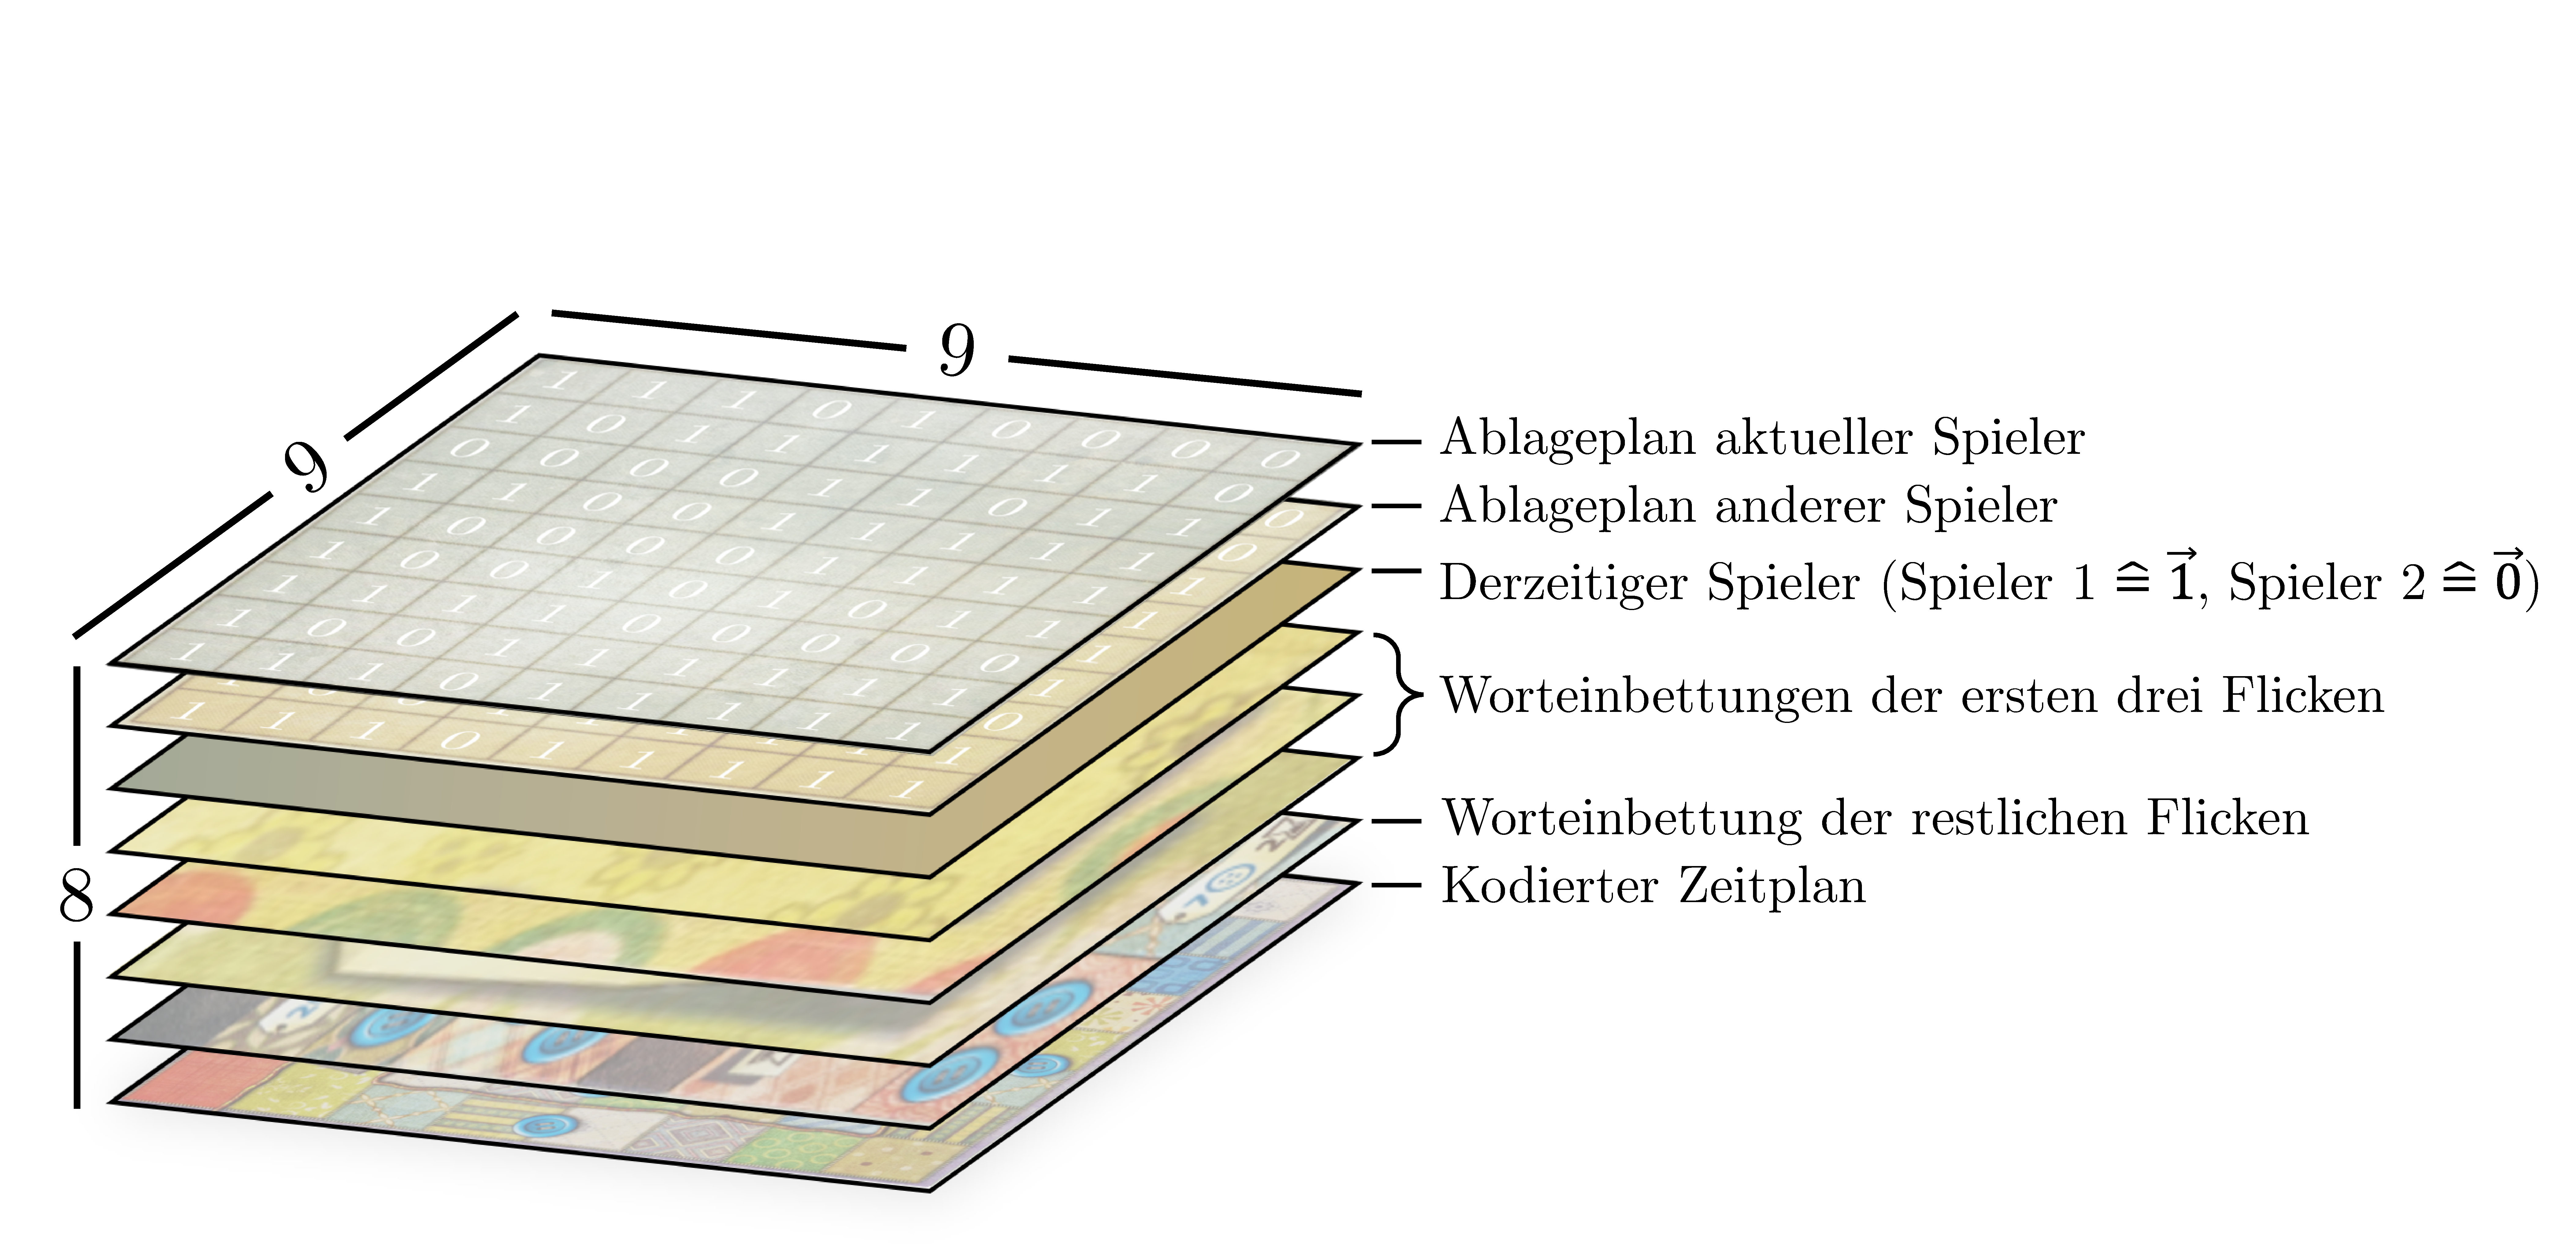
\includegraphics[width=\textwidth]{res/pictures/patch-zero-state.pdf}
    \vspace*{-0.45cm}
    \caption{Zustandskodierung von PatchZero}
    \label{fig:patch-zero-state}
\end{figure}
\vspace*{-0.25cm}

Zuerst wird der Ablageplan des aktuellen Spielers codiert. Dazu wird jedes mit Flicken belegte Feld in eine 1 umgewandelt und alle anderen Felder in eine 0. Danach folgt der Ablageplan des anderen Spielers mit der gleichen Kodierung. Daraufhin wird eine Ebene dafür verwendet dem Netzwerk den aktuellen Spieler mitzuteilen. Dabei steht eine $9\times 9$ gefüllte Ebene an Einsen für Spieler 1 und eine mit Nullen gefüllte Ebene für Spieler 2. Die originale AlphaZero Implementierung verwendet auch eine ganze Ebene für die Kodierung des aktuellen Spielers \cite[Anhang, S. 2]{2017.AlphaGoZeroPaper}. Dadurch, dass eine ganze Ebene für den aktuellen Spieler verwendet wird, können die lokalen Konvolutionsoperationen im Netzwerk, welche immer nur $n\times n\times 8$ Teilbereiche des Spielzustandes anschauen nachher jederzeit feststellen, welcher Spieler gerade an der Reihe ist. Dann werden in vier weiteren Ebenen die verfügbaren Flicken kodiert. Die ersten 3 verfügbaren Flicken werden jeweils in einer eigenen Ebene codiert, da diese auch alle drei einzeln für den derzeitigen Spieler zur Verfügung stehen. Sollte es einmal vorkommen, dass keine drei Flicken mehr zu Auswahl stehen, sondern zum Beispiel nur noch zwei, da alle anderen Flicken bereits vergeben sind, so wird die entsprechende Ebene mit Nullen gefüllt. Es ist aber unklar, ob das überhaupt im normalen Spiel vorkommen kann.

\vspace*{-5cm}
\pagebreak

\begin{figure}[!ht]
    \centering
    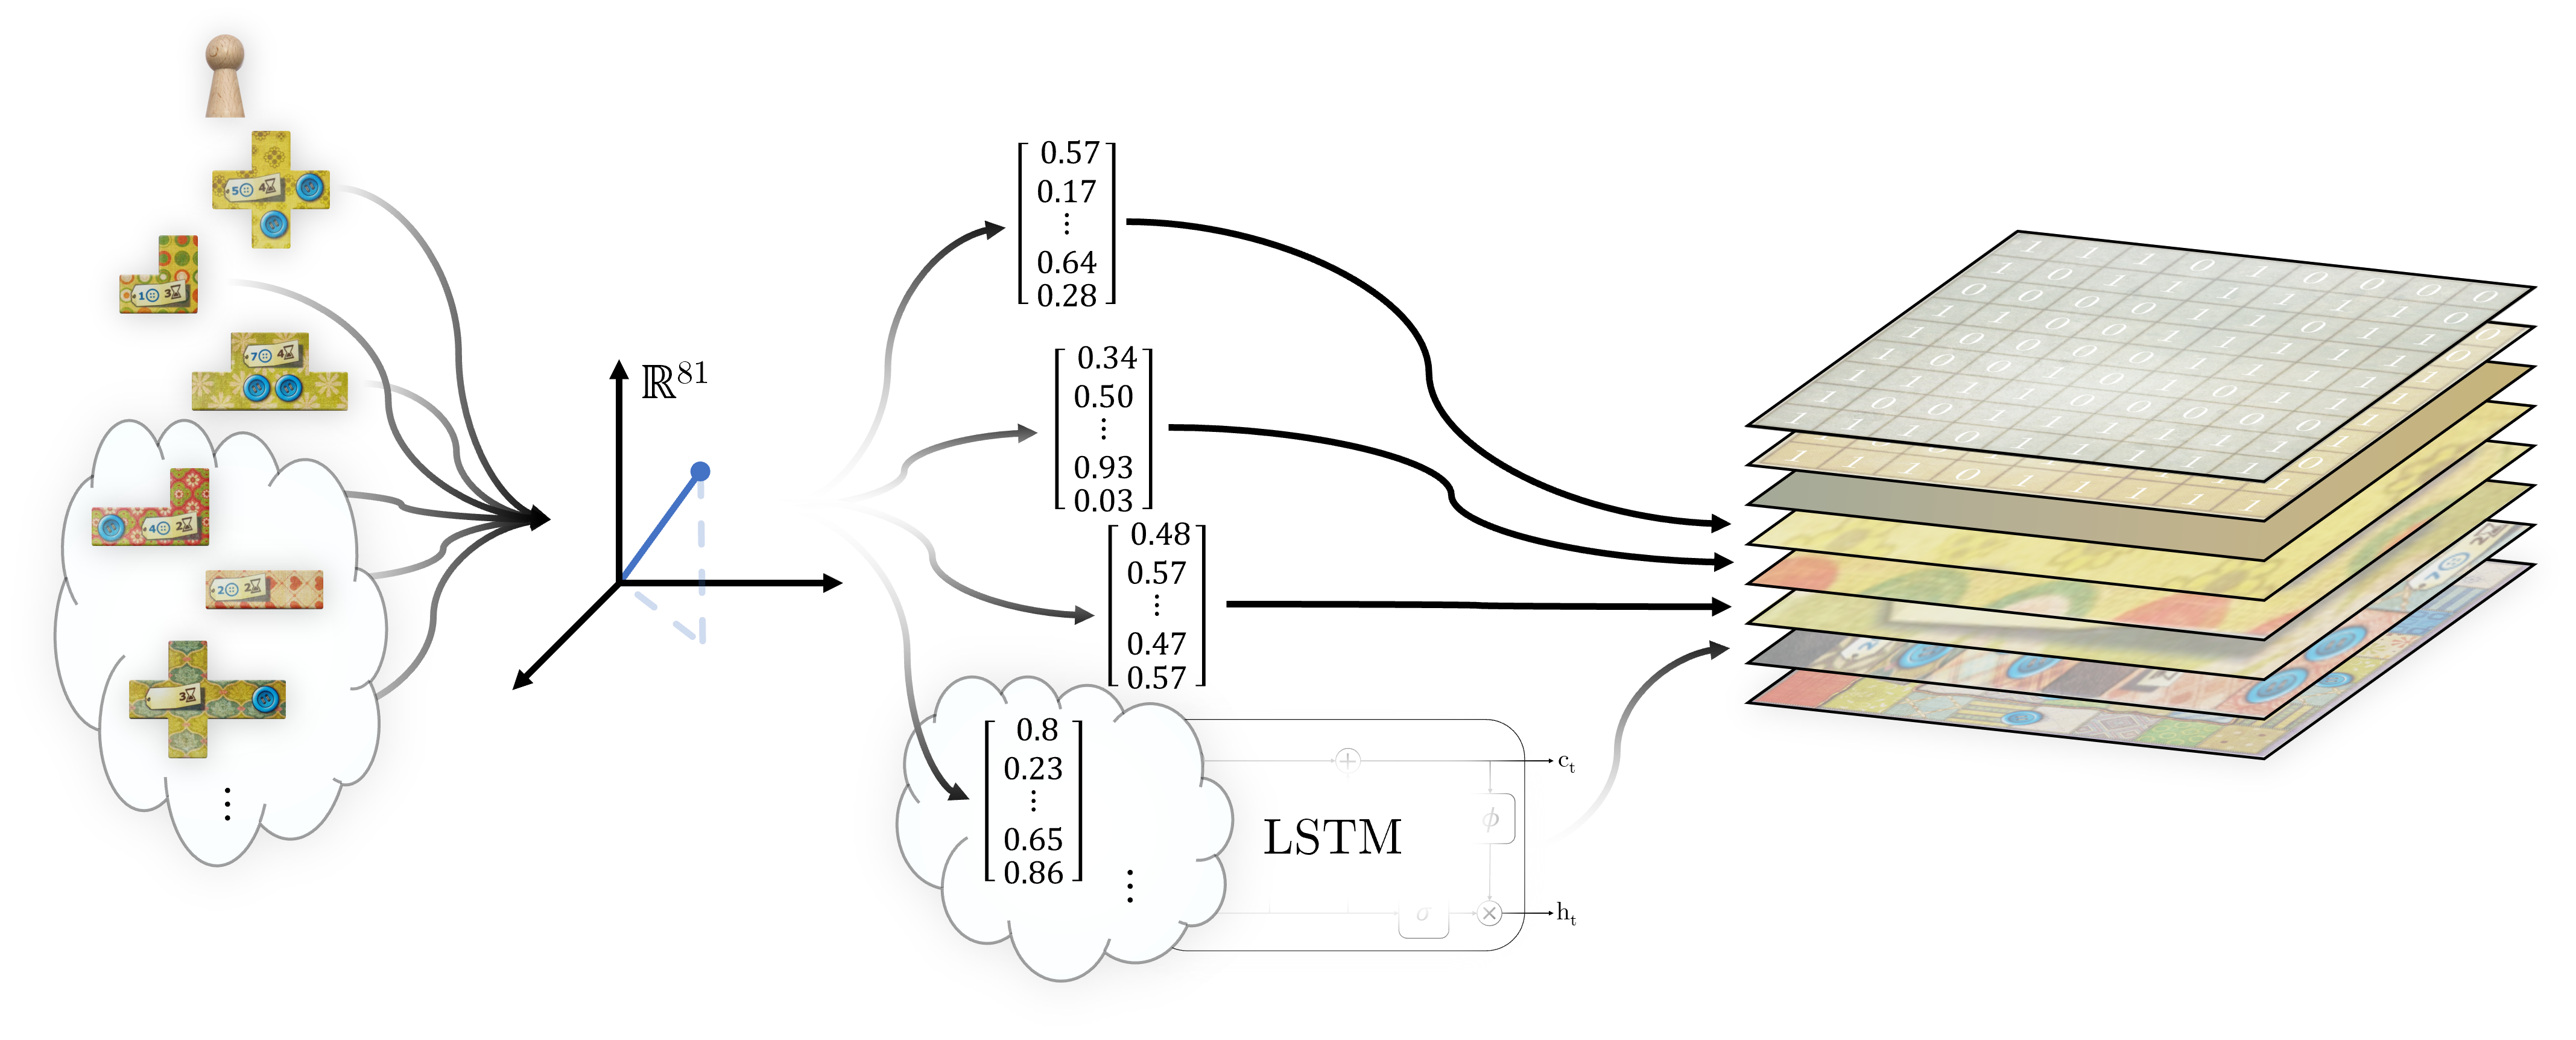
\includegraphics[width=\textwidth]{res/pictures/patch-embeddings.png}
    \vspace*{-0.5cm}
    \caption{Patch Embeddings}
    \label{fig:patch-embeddings}
\end{figure}
\vspace*{-0.25cm}

Da alle weiteren verfügbaren Flicken auch relevant sind, werden diese durch eine weitere Ebene repräsentiert. Die Anzahl der verfügbaren Flicken nimmt während dem Patchwork Spiel immer weiter stetig ab. Da das AlphaZero Netzwerk keinen Tensor von variabler Länge annehmen kann, müssen die restlichen Flicken zusammen in einer Ebene codiert werden. Um diese gemeinsame Kodierung hinzubekommen, wird ein rekurrentes \ac{LSTM} Netzwerk verwendet, was genau für diese Transformation mehrerer Eingaben in eine Ausgabe gemacht ist (Many-to-One) \cite{2015.RNN}. Dabei wird das \ac{LSTM} Netzwerk nacheinander mit den verfügbaren Flicken in falscher Reihenfolge aufgerufen, sodass beim ersten Aufruf der Flicken verwendet wird, der der Flicken ist, welcher am weitesten von der Spielfigur entfernt ist. Bei jedem Aufruf merkt sich das \ac{LSTM} intern einen Zustand, der auch in die Berechnung der Ausgabe eingeht. So kann final eine Ausgabe erzeugt werden, bei der alle Flicken zusammen mit ihrer Position innerhalb einer Ebene gemeinsam kodiert sind. Die Kodierung der einzelnen Flicken in eine $9\times 9$ Ebene wird nicht manuell vorgenommen, sondern es werden sogenannte Einbettungen verwendet. Dabei wird jeder Flicken-\ac{ID}, wie in Abbildung \ref{fig:patch-embeddings} zu sehen, ein Vektor mit 81 Einträgen zugeordnet. Dieser Vektor enthält dann die Werte für die passende Ebene im kodierten Spielzustand. Besonders ist hierbei, dass der Vektor mit allen 81 Werten durch das neuronale Netz gelernt wird, \dash während dem Training werden nach und nach wichtige Eigenschaften eines Flickens festgestellt und durch die Zahlen innerhalb des Vektors kodiert \cite{2023.PytorchEmbedding}. Somit kann das neuronale Netz selbst entscheiden, welche Eigenschaften relevant sind und muss nicht durch den Menschen vorgegebene Werte verwenden. Ein 81-dimensionaler Vektor sollte dabei auch ausreichen, um neben den Zeit-, Knopfkosten und dem Knopfeinkommen noch die Form und Ablagemöglichkeiten eines Flickens zu lernen.

\vspace*{-5cm}
\pagebreak

Zuletzt wird für die Spielzustandskodierung noch der Zeitplan mit allen relevanten Informationen in einer Ebene kodiert. Dazu werden verschiedene Eingaben durch ein neuronales Netzwerk mit 2 Schichten und einer \ac{ReLU} Aktivierungsfunktionen in eine 81 Zahlen lange Ausgabe transformiert, die anschließend in eine $9\times 9$ Ebene umgeformt wird. Die verschiedenen Eingaben setzen sich dabei wie folgt zusammen:

\begin{itemize}
    \item \vspace*{-0.1cm} Die Position des ersten Spielers auf dem Zeitplan, wobei die Werte nicht von 0 bis 54 gehen, sondern auf den Bereich $\left[0,1\right]$ normalisiert sind.
    \item \vspace*{-0.2cm} Die Position des zweiten Spielers auf dem Zeitplan mit der gleichen Normalisierung zu $\left[0,1\right]$.
    \item \vspace*{-0.2cm} Die Distanz zwischen beiden Spielern aus der Sicht des ersten Spielers von $\left[-6,6\right]$ normalisiert auf $\left[-1,1\right]$.
    \item \vspace*{-0.2cm} $9\times$ die Positionen der Knopfwertungen auf dem Zeitplan, normalisiert auf $(0,1]$.
    \item \vspace*{-0.2cm} $5\times$ die Positionen der Spezialflicken auf dem Zeitplan, normalisiert auf $(0,1)$.
    \item \vspace*{-0.2cm} Alle 54 Felder auf dem Zeitplan normalisiert auf $[0,1)$.
\end{itemize}
\vspace*{-0.1cm}

Diese menschlich ausgesuchten Angaben kann das PatchZero-Netzwerk durch die Transformation mit dem 2-Schichten-Netzwerk in für das Netzwerk besser geeignete Werte übertragen. So wird wie bei den Flicken der menschliche Bias nicht direkt an das Netzwerk übergeben.

\subsection{Netzwerk-Architektur}

\begin{wrapfigure}{r}{0.25\textwidth}
    \vspace*{-0.5cm}
    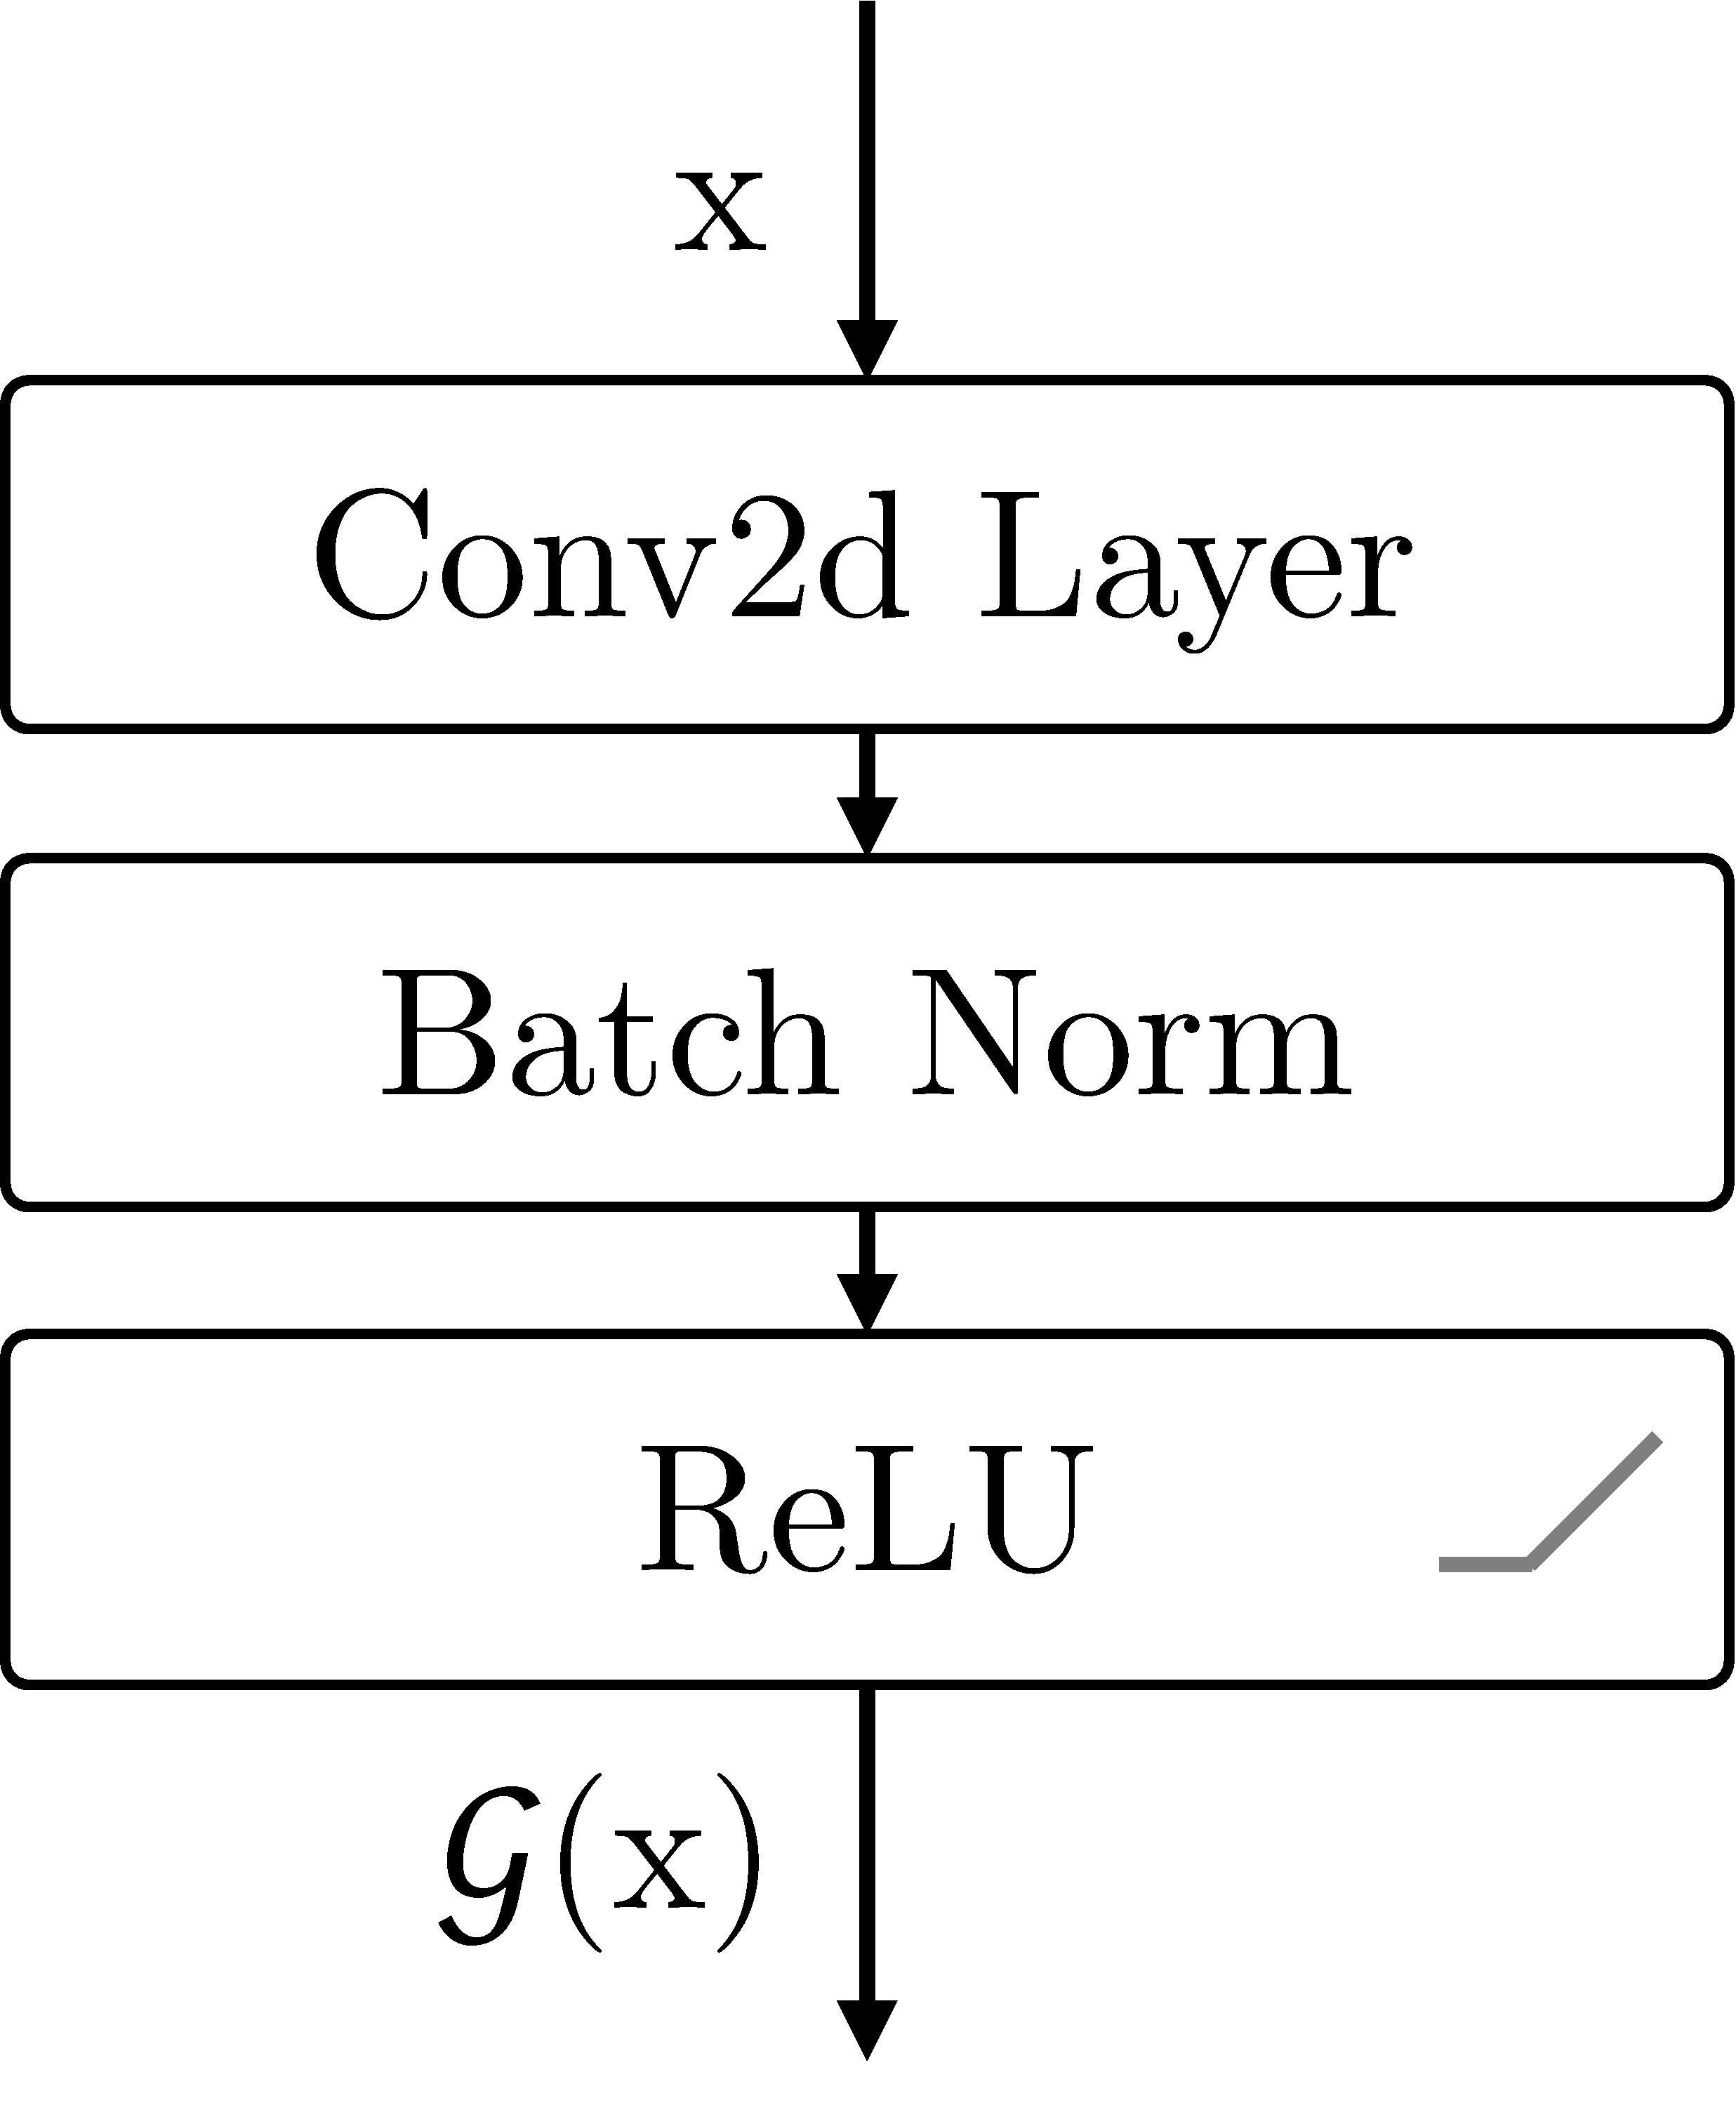
\includegraphics[width=0.23\textwidth]{res/pictures/conv-block.pdf}
    % \vspace{-10pt}
    % Das folgende ist ein Trick, um "Abbildung x.y" in eine
    % eigene Zeile zu packen. Der Text zwischen [ und ] steht
    % im Abbildungsverzeichnis. Der Text darunter wird
    % tatsächlich angezeigt.
    \centering
    \caption[Convolutional Block]{\unskip}
    Convolutional Block
    \label{fig:conv-block}
\end{wrapfigure}

Die in Abbildung \ref{fig:patch-zero-architecture} dargestellte Netzwerkarchitektur von PatchZero orientiert sich stark, an AlphaZero und \ac{Lc0}. Das Netzwerk nimmt den kodierten Spielzustand an und senden diesen durch einen in \ref{fig:conv-block} gezeigten \enquote{Convolutional Block}. Dieser Convolutional-Layer (Conv2d) betrachtet $3\times 3 \times 8$ Regionen innerhalb des kodierten Zustands und extrahiert somit lokale Informationen. Daraufhin folgt eine Batch Normalisierung, um die Werte innerhalb des Netzwerks klein zu halten. So lässt sich das Netzwerk nachher schneller trainieren \cite{2018.BatchNorm}. Die Aktivierungsfunktion \ac{ReLU} wird verwendet, um Nichtlinearitäten in das Netzwerk einzuführen.

\vspace*{-5cm}
\pagebreak

\begin{figure}[!ht]
    \centering
    \includegraphics[width=\textwidth]{res/pictures/patch-zero-architecture.pdf}
    \caption{Netzwerkarchitektur von PatchZero}
    \label{fig:patch-zero-architecture}
\end{figure}

\begin{wrapfigure}{l}{0.3\textwidth}
    \vspace*{-0.375cm}
    \centering
    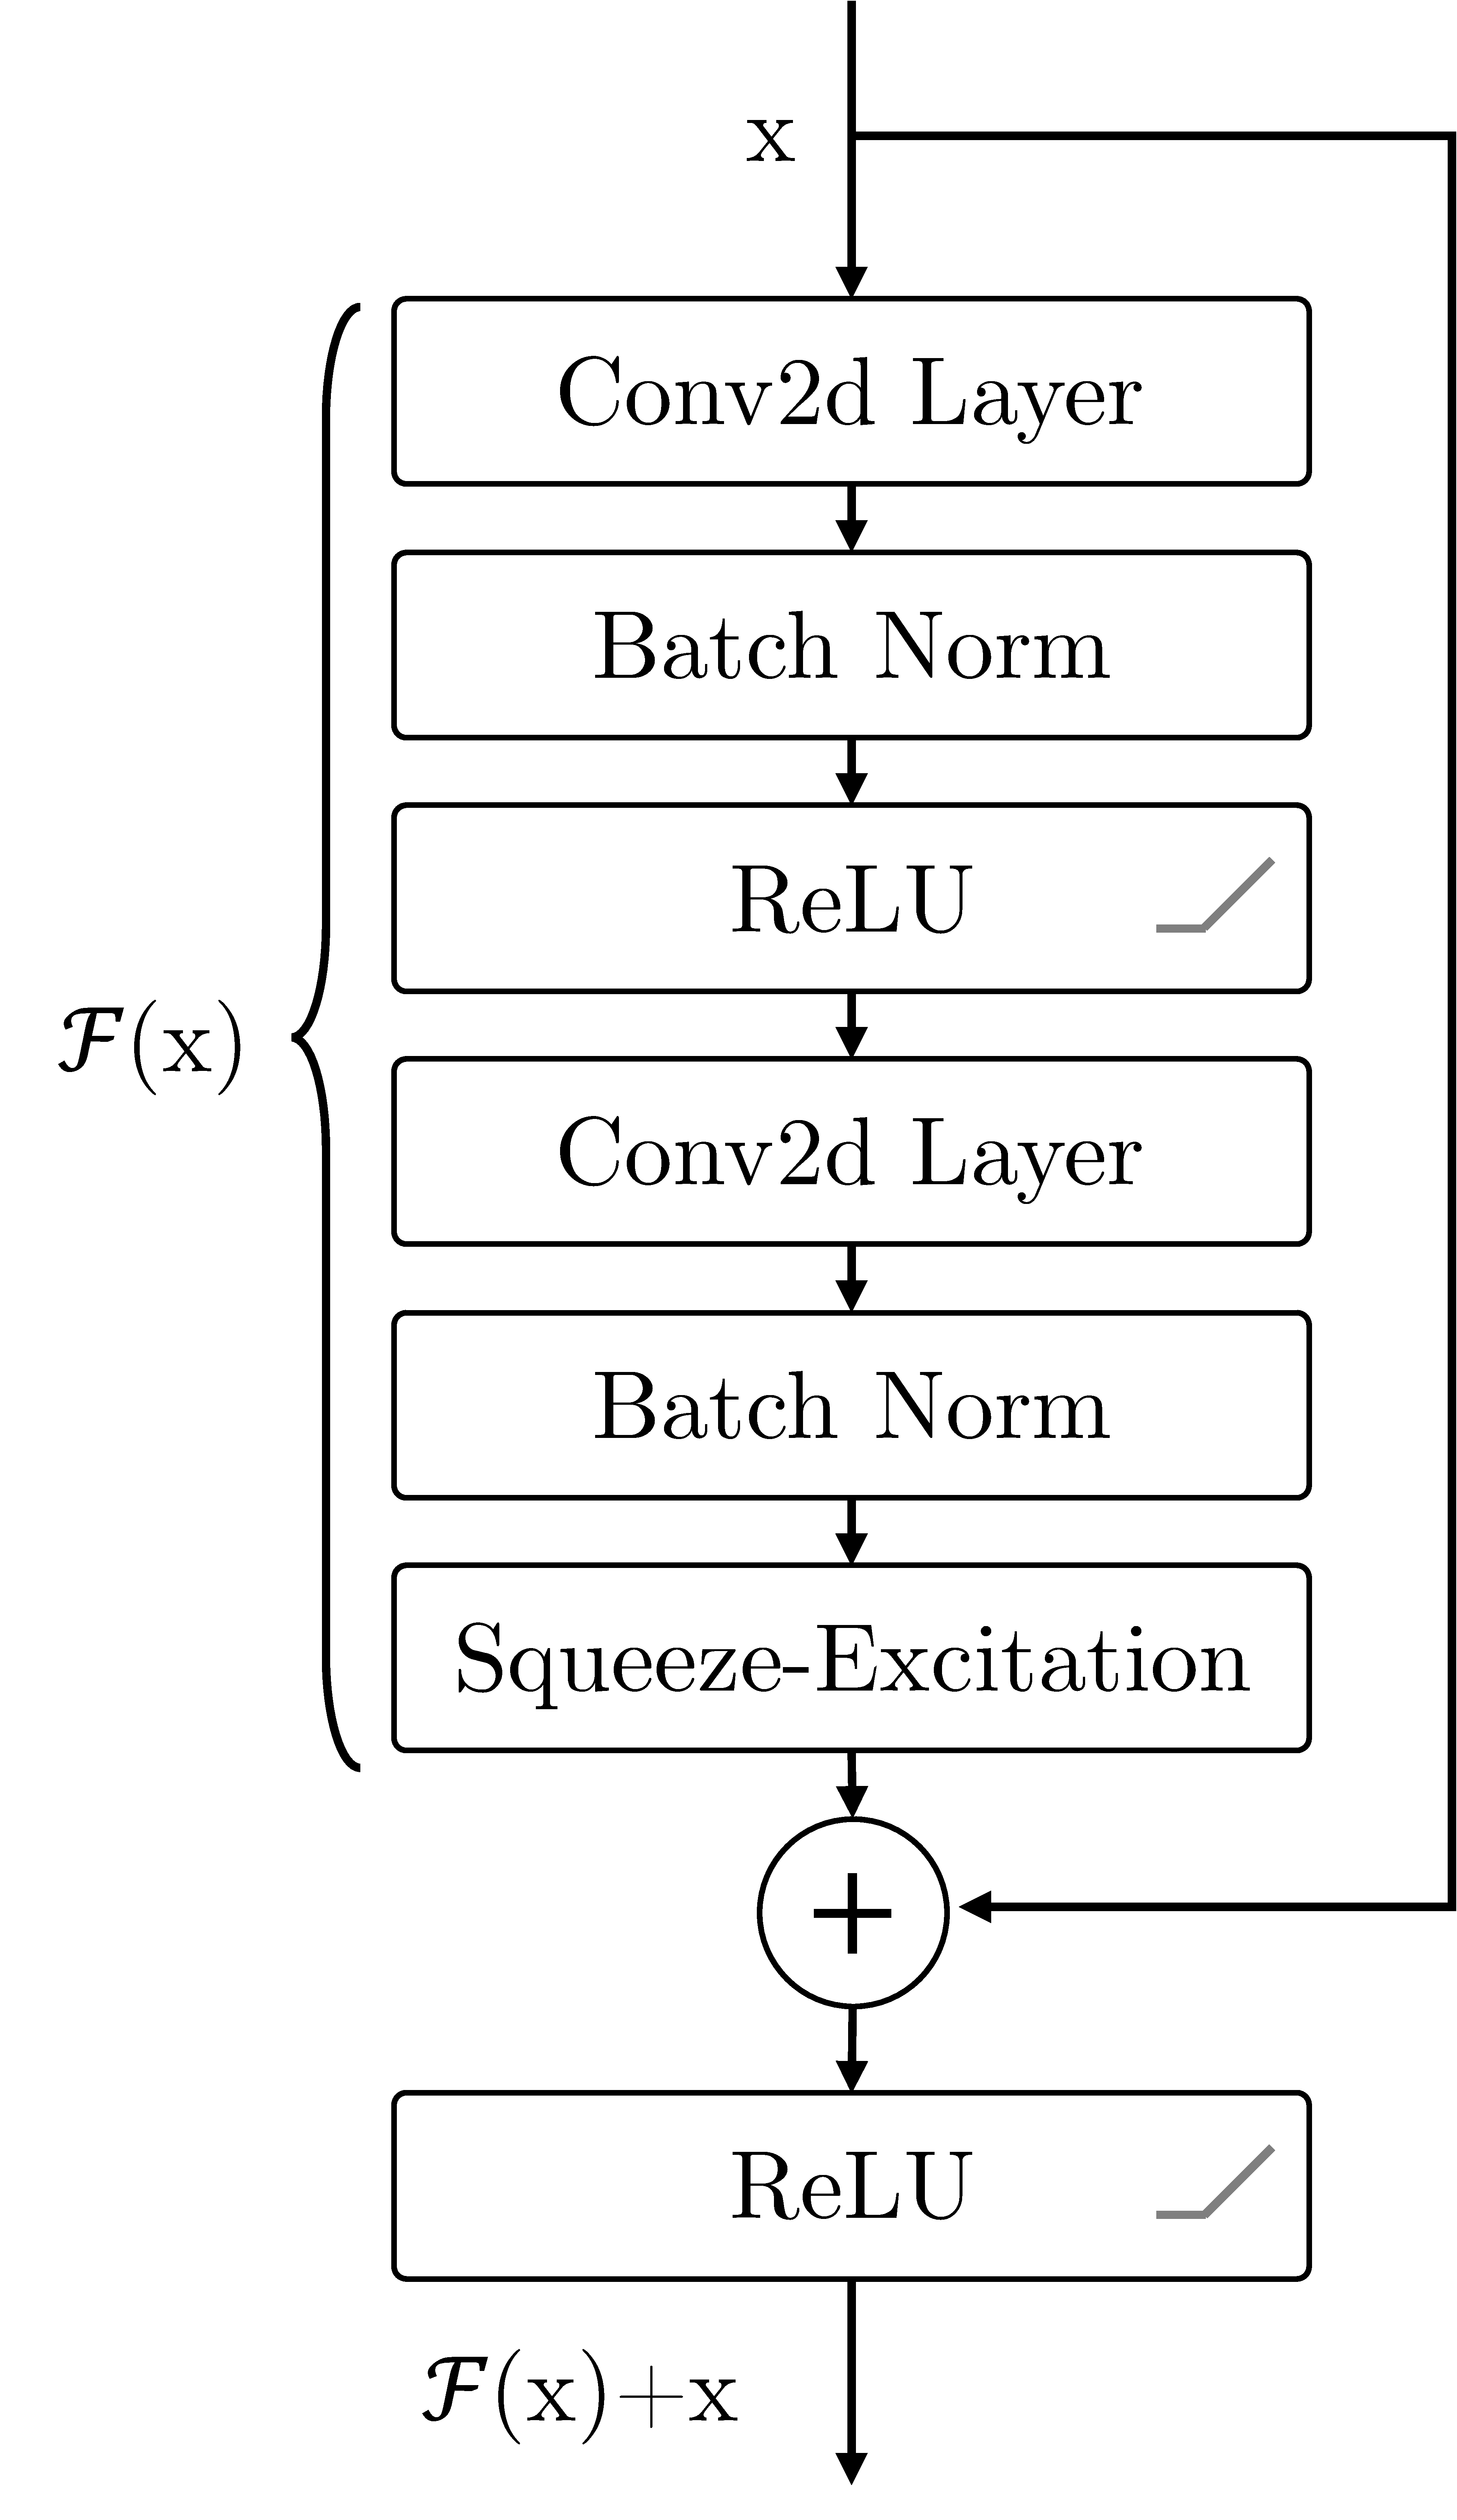
\includegraphics[width=0.28\textwidth]{res/pictures/res-block.pdf}
    \vspace*{-5pt}
    \caption[Residual Block]{\unskip}
    Residual Block
    \label{fig:resblock}
    \vspace*{-2.5cm}
\end{wrapfigure}

Anschließend werden die Daten durch einen Stapel an \enquote{Residual Block} Elementen geleitet. Diese \enquote{Residual Blöcke} sind dabei ähnlich aufgebaut wie der \enquote{Convolutional Block}, um Informationen aus dem Datenstapel zu extrahieren (Abbildung \ref{fig:resblock}). Die Besonderheit dabei ist, dass neben dem eigentlichen Netzwerk auch die Eingabe $x$ über eine weitere

\begin{minipage}{0.67\textwidth}
    % \textwidth = 449.55371pt
    % \vspace*{-0.05cm}
    \begin{addmargin}[144.866113pt]{0em}
        Verbindung bis an das Ende unverändert durchgereicht wird. So muss anstatt der kompletten Ausgabe nur noch die Differenz $\mathcal{F}\left(x\right) = \mathcal{H}\left(x\right) - x$ zwischen der Eingabe $x$ und der Ausgabe $\mathcal{H}\left(x\right)$ gelernt werden, was das Lernen in tiefen neuronalen Netzwerken vereinfacht
    \end{addmargin}
    \cite[S. 3]{2015.ResNet}. In PatchZero sind 10 dieser \enquote{Residual Blöcke} hintereinandergeschaltet, wobei jeder Block 64 einzelne $3\times 3$ Konvolutionsfilter besitzt, um lokale Informationen zu extrahieren. Diese lokalen Informationen werden in den späteren Schichten immer mehr zu globalen Informationen zusammengefasst, woraus die Evaluation der Spielposition entsteht.
\end{minipage}
\begin{minipage}{0.33\textwidth}
    \centering
    \captionsetup{type=figure}
    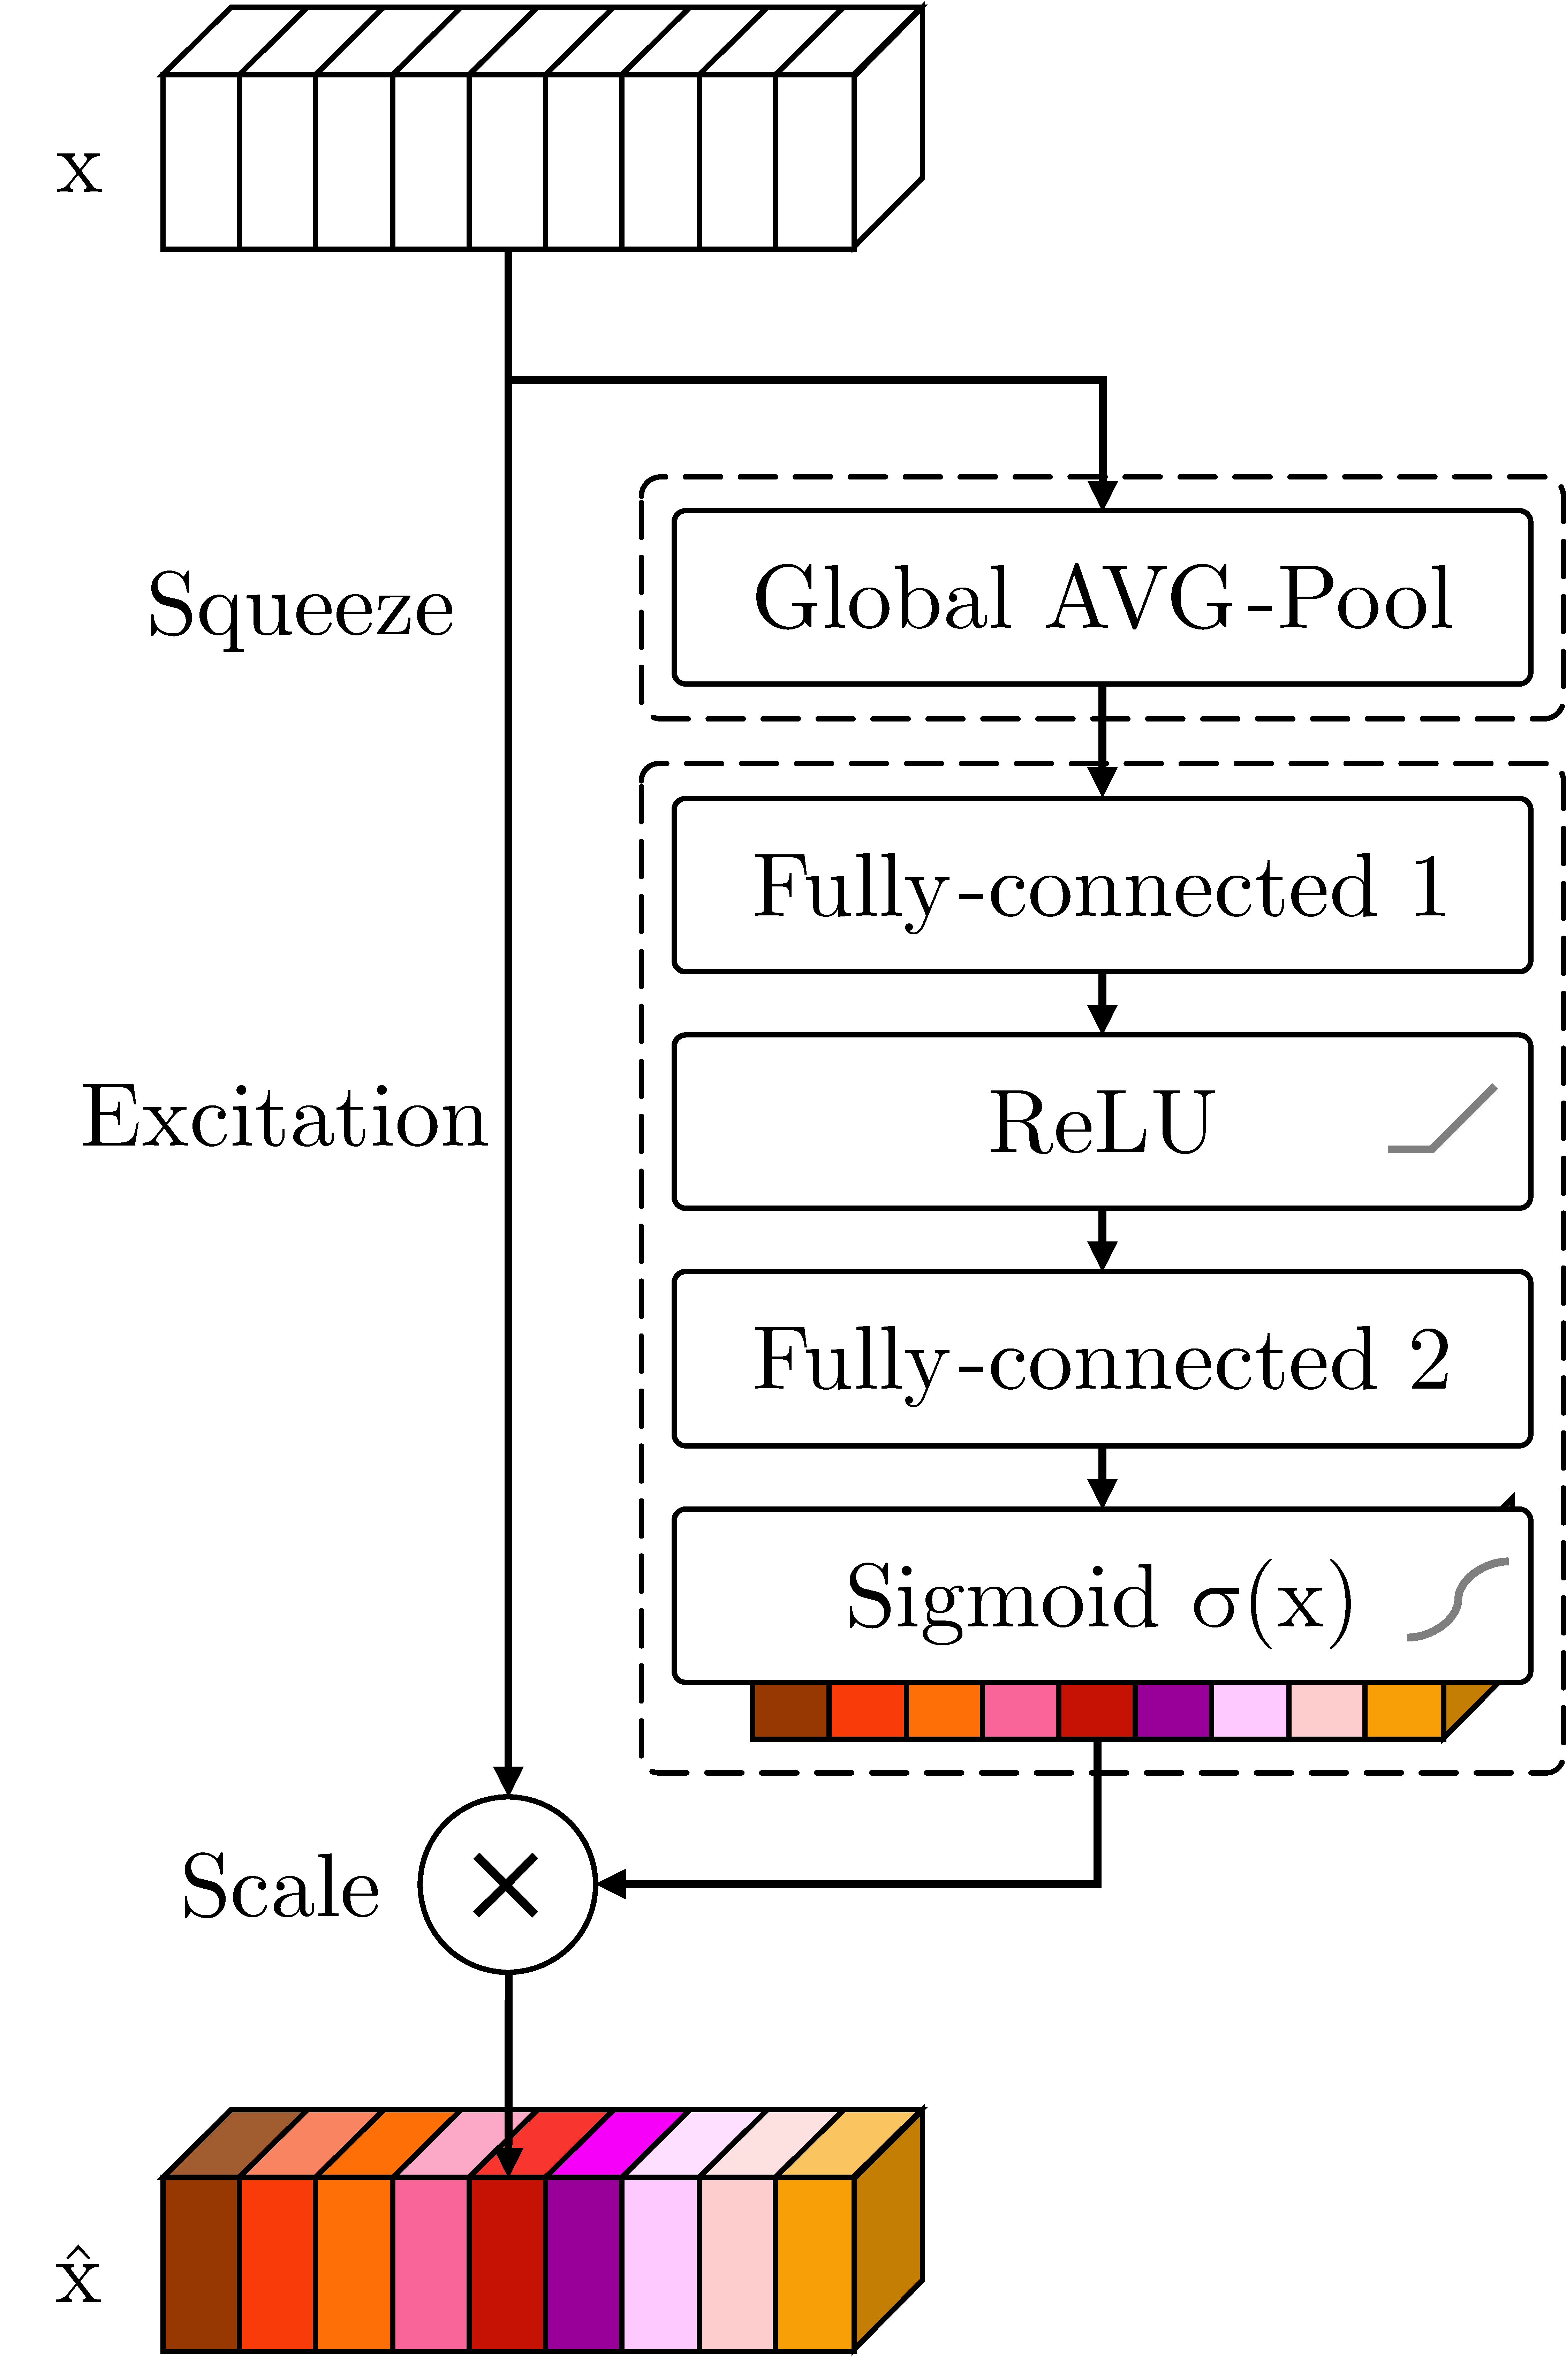
\includegraphics[width=0.95\linewidth]{res/pictures/squeeze-and-excitation-block.pdf}
    \captionof{figure}[Squeeze \& Excitation Block]{\unskip}\label{fig:squeeze-and-excitation-block}
    Squeeze \& Excitation Block
\end{minipage}

\vspace*{-10cm}
\pagebreak

Weiterhin verwendet PatchZero in den \enquote{Residual Blöcken} noch eine von \ac{Lc0} eingeführte Erweiterung mit den in Abbildung \ref{fig:squeeze-and-excitation-block} dargestellten \enquote{Squeeze \& Excitation} Blöcken \cite{2020.Lc0NetworkTopology}. Dieser Block erweitert eine normale Konvolution mit mehreren Filtern, indem die einzelnen Filterkanäle nach ihrer Bedeutung in der Ausgabe skaliert werden \cite[S. 1]{2019.SqueezeandExcitation}.

Im letzten Schritt wird das Netzwerk in einen \emph{Value Head} und ein \emph{Policy Head} aufgeteilt. Diese können somit zwei voneinander unabhängige Netzwerkausgaben produzieren. Zum einem wird vom \emph{Value Head} eine Approximation der Evaluation der Spielposition aus Sicht des derzeitigen Spielers produziert und andererseits erzeugt der \emph{Policy Head} die Wahrscheinlichkeitsverteilung, wie gut es ist einzelne Aktionen ausgehend vom Spielzustand auszuführen.

\vspace*{-0.55cm}
\begin{figure}[!ht]
    \centering
    \includegraphics[width=0.7\textwidth]{res/pictures/value-and-policy-head.pdf}
    \\
    \begin{minipage}{.49\textwidth}
        \centering
        \captionof{figure}[Value Head von PatchZero]{\unskip}
        Value Head von PatchZero
        \label{fig:value-head}
    \end{minipage}
    \hfill
    \begin{minipage}{.49\textwidth}
        \centering
        \captionof{figure}[Policy Head von PatchZero]{\unskip}
        Policy Head von PatchZero
        \label{fig:policy-head}
    \end{minipage}
\end{figure}

Der in Abbildung \ref{fig:value-head} dargestellte \emph{Value Head} sendet die Daten dabei durch mehrere Fully-connected Layer, bevor eine finale Evaluation mittels der $\tanh$ Funktion ausgegeben wird. Die Tangens Hyperbolicus Funktion stellt dabei sicher, dass die Ausgabe in den Bereich von $\left[-1,1\right]$ fällt, wobei eine $1$ für das Gewinnen und eine $-1$ für das Verlieren des derzeitigen Spielers steht.

\pagebreak

Im Gegensatz dazu wird beim \emph{Policy Head} (Abbildung \ref{fig:policy-head}) die Eingabe nicht auf einen Wert reduziert, sondern es wird ein Vektor an Ausgaben produziert, mit jeweils einer Zahl für jede mögliche \hyperref[text:natural-action-id]{\code{NaturalActionId}}. Durch die in \ref{eqn:softmax} die \emph{Softmax} Funktion werden die Daten vor der Ausgabe stetig in eine Wahrscheinlichkeitsverteilung transformiert.

\vspace*{-0.5cm}
\begin{align}
    \label{eqn:softmax}
    \sigma\left(\vec{x}\right): & \begin{cases}
        [\min \vec{x}, \max \vec{x}] \to \left[0,1\right] \\
        \sigma\left(\vec{x}_i\right)= \frac{e^{\vec{x}_i}}{\sum_{j=1}^n e^{\vec{x}_j}}
        \end{cases} \\
        &   \text{mit } \forall a,b: a<b \implies \sigma\left(a\right) < \sigma\left(b\right) \notag
\end{align}
\vspace*{-1.2cm}

Vor der Netzwerkevaluation wird von einer Spielposition jede aus dem Spielzustand mögliche \hyperref[text:action-id]{\code{ActionId}} bestimmt. Dann wird eine Zuordnung zwischen \hyperref[text:action-id]{\code{ActionId}} und passender \hyperref[text:natural-action-id]{\code{NaturalActionId}} erstellt, da diese die Ausgabe des neuronalen Netzes darstellen. Bei der Ausgabe des neuronalen Netzes kann es nun sein, dass Aktionen, welche nicht ausgeführt werden können, trotzdem eine Wahrscheinlichkeit von nicht Null erhalten. Aus diesem Grund muss die Ausgabe des \emph{Policy Head} wie in Quellcode \ref{code:patch-zero-transform-output} gezeigt noch mit einem Tensor multipliziert werden, der bei allen verfügbaren Aktionen eine Eins als Eintrag besitzt und ansonsten Null. Um die Wahrscheinlichkeitsverteilung der Ausgabe zu erhalten, müssen wieder alle Einträge durch die Gesamtsumme geteilt werden.

\vspace*{-0.1cm}
\lstinputlisting[
    label={code:patch-zero-transform-output},
    caption={Ausgabentransformation bei PatchZero},
    captionpos=b,
    language=Rust,
    firstline=0,
]{res/code/patch-zero-transform-output.rs}
\vspace*{-0.2cm}

Die Ausgaben des \emph{Value Heads} und des \emph{Policy Heads} sind dabei ein- bzw. zweidimensional, anstatt wie zu erwarten nur ein Skalar bzw. ein eindimensionaler Vektor. Das ist der Fall, da das neuronale Netz neben den Ausgabedimensionen noch eine weitere Dimension, die Minibatch-Dimension, besitzt. Diese weitere Dimension wird zur gleichzeitigen Evaluation mehrerer Spielzustände eingesetzt. Dies wird im nachfolgenden Abschnitt »\nameref{section:erstellung-ansatz-d-parallelisierung}« noch genauer besprochen.

\vspace*{-5cm}
\pagebreak

Um nach der Evaluation mit der Expansions- und Backpropagationsphase fortführen zu können, wird zuletzt eine Rücktransformation der Ausgabe, bei der es sich um die Wahrscheinlichkeiten der \hyperref[text:natural-action-id]{\code{NaturalActionId}} handelt, in eine \hyperref[text:action-id]{\code{ActionId}} vorgenommen, sodass die neuen Spielzustände nach der Anwendung einer Aktion erstellt werden können.

\subsection{Parallelisierung}
\label{section:erstellung-ansatz-d-parallelisierung}

Im Gegensatz zum \ac{MCTS} Spieler wird bei PatchZero die \hyperref[text:tree-parallelization]{\emph{Tree Parallelisierung}} verwendet, um eine Suche über mehrere Kerne bereitzustellen. Diese Parallelisierungsart wird auch von der originalen AlphaZero Implementierung mit gutem Grunde verwendet. Die Ausführung eines neuronalen Netzes ist umso effizienter, umso mehr Datensätze das Netz auf einmal als Eingabe erhält. Zwar ist insgesamt die Zeit, die das neuronale Netz für die Forwardpropagation, also der Transformation der Eingaben in die Ausgaben, braucht höher, jedoch wird die Zeit die durchschnittlich für einen Datensatz benötigt wird geringer. Dies ist der Fall, da sich der Aufwand für die Parallelisierung verschiedener Operationen wie Matrixmultiplikation erst bei größeren Eingaben für eine Geschwindigkeitserhöhung der Forwardpropagation lohnt. \cite[S. 201f.]{2021.NetworkParallelization}

Deswegen gibt es beim PatchZero Spieler 8 Threads, die gleichzeitig in einem Suchbaum Iterationen durchführen. Ein Thread startet bei dem Wurzelknoten und sucht sich mithilfe der PUCT Tree Policy einen Pfad durch den Baum bis zu einem noch nicht expandierten Knoten. Dabei wird wie innerhalb der \hyperref[text:tree-parallelization]{\emph{Tree Parallelisierung}} beschrieben bei jedem Knoten ein \emph{Virtual Loss} hinzugefügt. Ist der Thread beim nicht expandierten Knoten angekommen, wird der entsprechende Spielzustand in die nächste Minibatch Evaluation des Netzwerks aufgenommen. Ist eine gewisse Anzahl an Minibatch-Einträgen erreicht (im PatchZero Spieler standardmäßig 20), führt der Thread, der den letzten Eintrag in den Minibatch eingefügt hat, die Evaluation aller Einträge mittels des neuronalen Netzes aus. Dieser Thread übernimmt dann im Anschluss auch die Backpropagation aller Ergebnisse durch den Baum, sowie das Entfernen der \emph{Virtual Losses}. In der Zwischenzeit suchen die anderen Threads weiter im Baum und fügen neue Knoten bzw. Zustände in die Minibatch Liste ein. Ist die Zeit vorbei, wird am Ende noch zwangsweise eine letzte Netzwerkevaluation durchgeführt, um auch die ausstehenden Einträge zu evaluieren. Der gesamte Quellcode einer Minibatch Evaluation ist in Anhang \ref{code:patchzero-mini-batch-evaluation} zu sehen.

\subsection{Training des Netzwerks}

\begin{figure}[!ht]
    \centering
    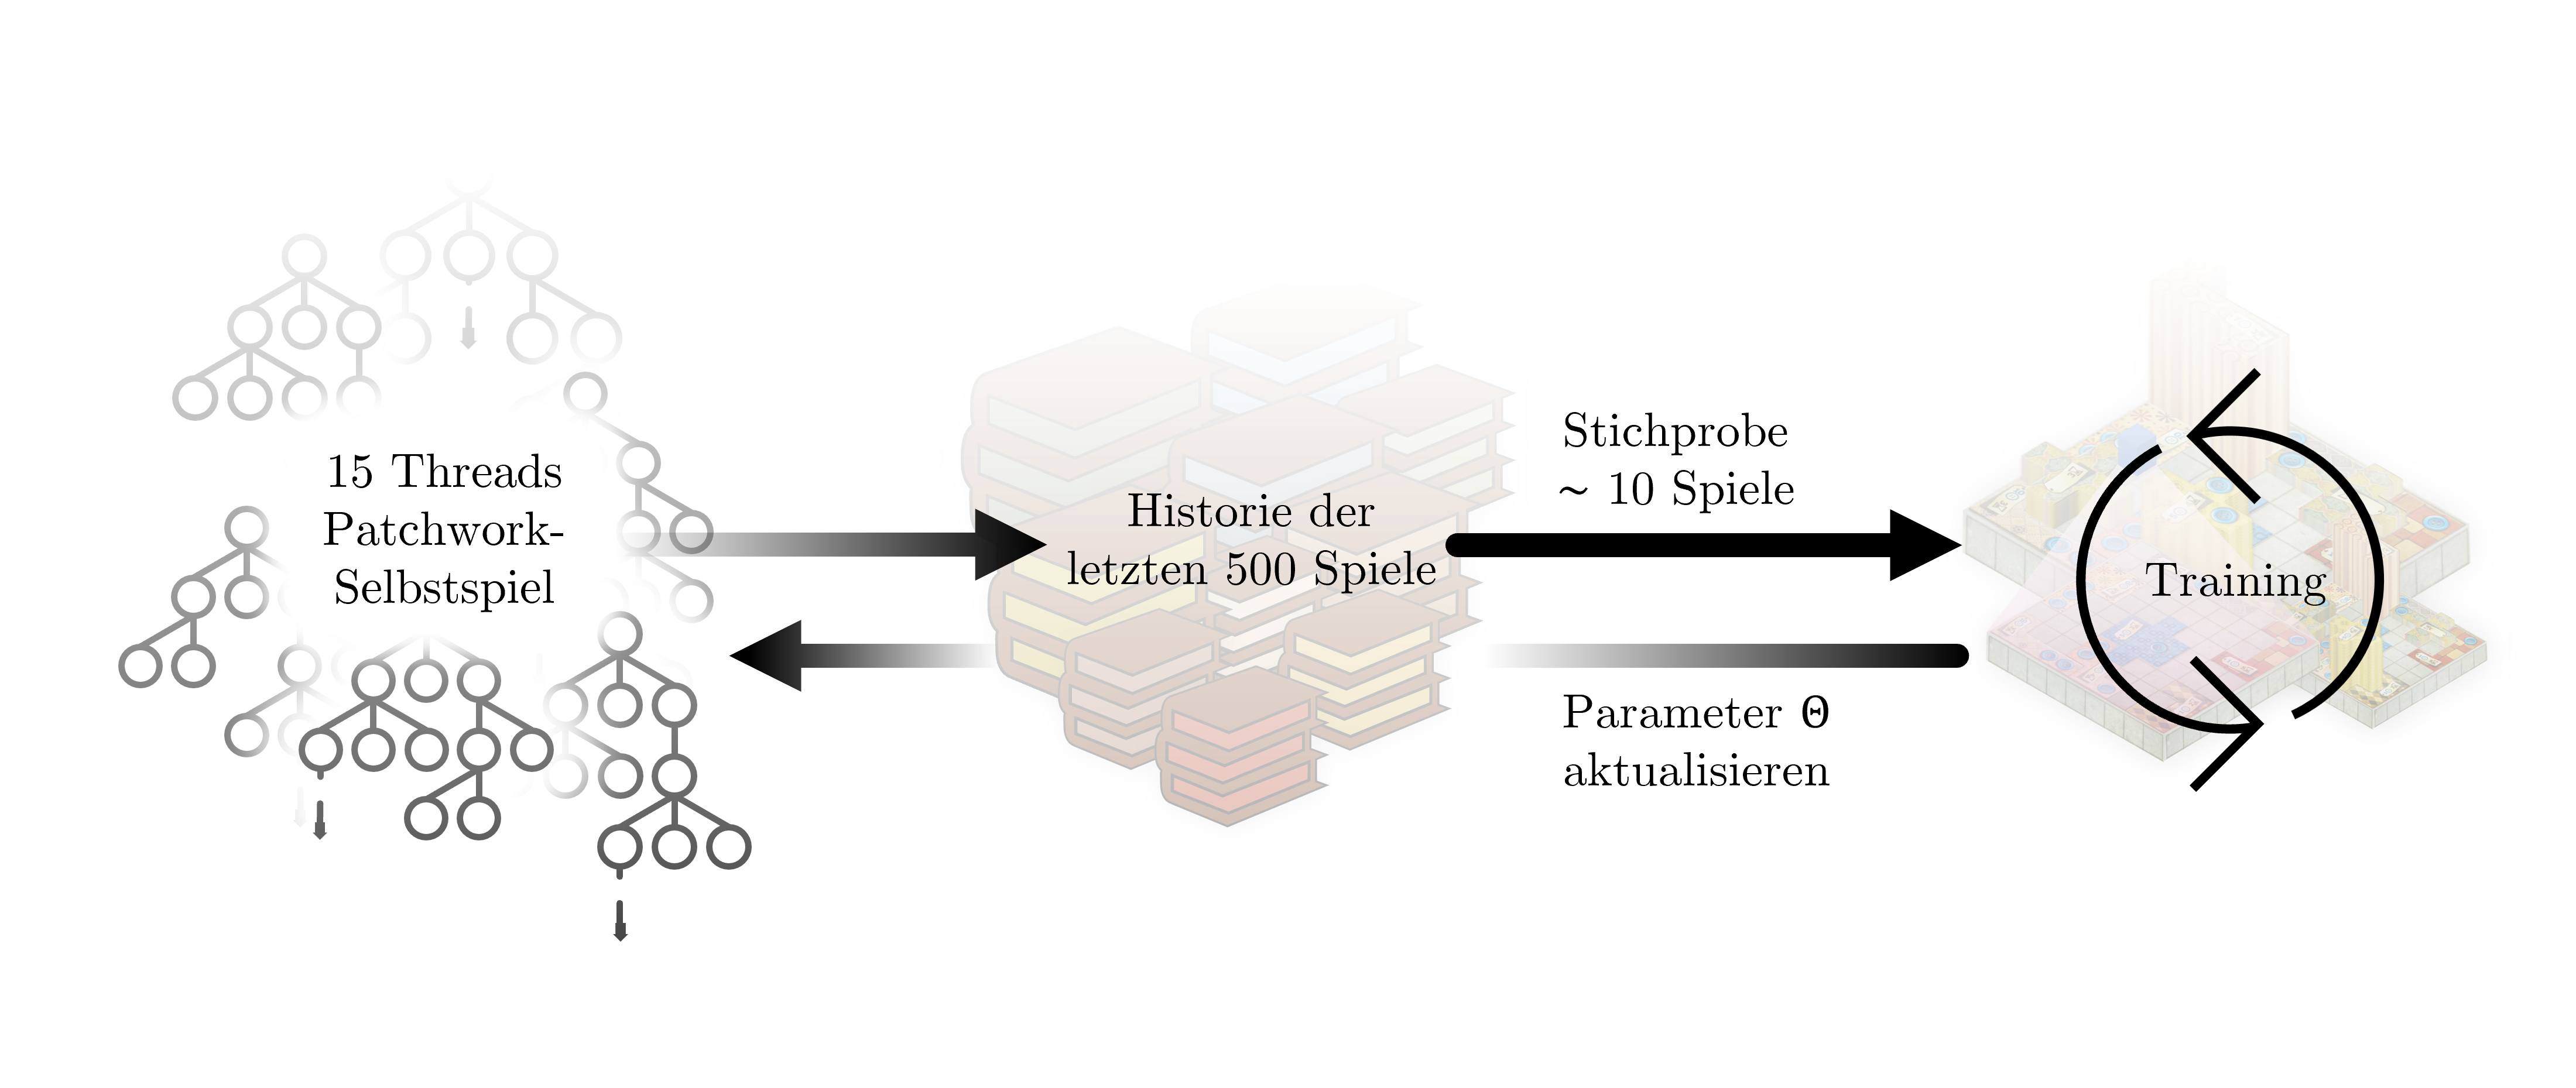
\includegraphics[width=\textwidth]{res/pictures/patch-zero-train.png}
    \caption{Trainingsprozess von PatchZero}
    \label{fig:patch-zero-train}
\end{figure}

Damit das neuronale Netzwerk $f_\theta$ sinnvolle Ausgaben für die Evaluation und die Aktionenwahrscheinlichkeiten eines Spielzustands liefern kann, ist ein Training mit Daten notwendig. Alle Gewichte $\theta$ des Netzwerks werden zuerst zufällig initialisiert. Diese Parameter werden dann in Laufe des in Abbildung \ref{fig:patch-zero-train} zu sehenden bestärkenden Lernprozesses aktualisiert, indem als Trainingsdaten Spieldaten verwendet werden, welche durch Patchwork-Spiele von PatchZero gegen sich selbst mit dem Netzwerk $f_\theta$ entstanden sind.

Die Trainingsdaten werden dabei bei PatchZero von 15 gleichzeitig ablaufenden Threads generiert. Diese spielen immer wieder Patchwork Spiele von 2 PatchZero Spielern gegeneinander. Dabei hat jeder PatchZero 1000 Monte Carlo Iterationen, um sich für einen Zug zu entscheiden. Die Evaluation des Netzwerks wird dabei vollständig auf der \ac{CPU} ausgeführt, da eine Übertragung der Eingangsdaten auf eine \ac{GPU} länger benötigt, als die $12\acs{ms}$, in der das Netzwerk die Evaluation erzeugt.

Die PatchZero Spieler spielen dabei zum Großteil wie im normalen Spiel mit einigen kleineren Änderungen, um das Training zu erleichtern. Um die Exploration zu fördern und so auch unbekannte neue Situationen zu erreichen, wird nicht mehr die Aktion ausgewählt, welche nach 1000 Iterationen am meisten Besuche vorliegen hat, sondern es wird nach der in Term \ref{eqn:patch-zero-train-policy} dargestellten Formel entschieden.

\begin{align}
    \label{eqn:patch-zero-train-policy}
    \pi\left(a\,|\,s_0\right) = \left(\frac{\phantom{ab\sum} \mathsf{Visits}\left[s_1 \gets s_0\left(a\right) \right]}{\phantom{ab}\sum\limits_{\mathclap{b\, \in\, \text{Actions}}} \mathsf{Visits}\left[s_1 \gets s_0\left(b\right) \right]}\right)^{\text{\Large $\frac{1}{\tau}$}}
\end{align}

Dabei ist die Wahrscheinlichkeit eine Aktion $a$ vom Wurzelknoten $s_0$ ausgehend auszuwählen $\pi\left(a\,|\,s_0\right)$ immer noch proportional zur Anzahl der Besuche. So ergibt sich für alle möglichen Aktionen eine Wahrscheinlichkeitsverteilung, aus der die tatsächlich gespielte Aktion als Stichprobe ausgewählt wird. Bei der Temperatur $\tau$ handelt es sich dabei um einen Hyperparameter, der in PatchZero auf $1{,}25$ gesetzt ist. Je größer $\tau$ ist, desto näher rücken die Wahrscheinlichkeiten aller Aktionen zusammen, \dash PatchZero wird experimentierfreudiger und wählt auch öfters schlechtere Aktionen. $\tau \to 0$ entspricht wieder dem $\argmax$ aller Aktionen, also einer Auswahl der besten Aktion. Nach $35$ \hyperref[text:ply]{\emph{Plys}} wird $\tau$ bei PatchZero ähnlich wie bei AlphaZero auf genau solch eine Infinitesimalzahl gesetzt, um kompetitiv zu Spielen und so das Beste zu erwartende Ergebnis zu erspielen \cite[Anhang, S. 2]{2017.AlphaGoZeroPaper}. Zusätzliche Exploration wird weiterhin durch das Hinzufügen von Dirichlet Rauschen im Wurzelknoten erreicht. Die \emph{A-priori} Wahrscheinlichkeit wird durch $\pi_{Root}\left(s_0\,|\,a\right) = (1 - \varepsilon) \cdot \pi\left(s_0\,|\,a\right) + \varepsilon\eta$ gegeben, wobei $\eta \sim \operatorname{Dir}(0{,}2)$ und $\varepsilon = 0{,}25$ \cite[Anhang, S. 2]{2017.AlphaGoZeroPaper}. Dieses zusätzliche Rauschen zwingt den PatchZero Spieler während dem Selbstspiel alle möglichen Aktionen auszuprobieren, erlaubt aber weiterhin das genauere erforschen von besseren Aktionen.

Sobald ein Spiel fertig gespielt ist, werden alle Zustände zusammen mit dem Ergebnis in einer Historie abgelegt. Diese Historie umfasst immer die letzten 500 Patchwork Spiele, die durch die Threads erzeugt wurden. Die Begrenzung dient dazu alte Trainingsdaten mit der Zeit zu entfernen, da diese mithilfe von alten Parametern $\theta$ des Neuronalen Netzes generiert wurden und somit nicht mehr direkt mit der aktuellen Spielweise in Verbindung stehen müssen. Aus der Historie an Spielen nimmt dann ein weiterer Thread immer wieder eine Stichprobe von 10 Spielen. Diese Stichprobe wird dann zum Training des Netzwerkes verwendet. Dabei wird über 10 Epochen trainiert und eine Batch Size von 128 \hyperref[text:ply]{\emph{Plys}} verwendet, \dash jedes Spiel wird 10-mal verwendet (Epochen), um die Parameter $\theta$ des Netzwerks zu aktualisieren. Die Batch Size bedeutet, dass immer 128 \hyperref[text:ply]{\emph{Plys}} aus allen 10 Spielen herausgegriffen werden und gemeinsam für eine Aktualisierung von $\theta$ verwendet werden.  Trainiert wird wie bei neuronalen Netzen üblich über das Gradientenabstiegsverfahren, indem die in \ref{eqn:patch-zero-loss-function} gezeigte \emph{Loss}-Funktion minimiert wird.

\begin{align}
    \label{eqn:patch-zero-network-output}
    (\mathcal{V}, \pi) &= f_\theta\left(s\right) \\
    \label{eqn:patch-zero-loss-function}
    \text{Loss} &= \underbrace{\left(z - \mathcal{V}\right)^2}_{\acs{MSE}}\:\,\mspace{1mu} \underbrace{-\: p^\mathsf{T}\, \ln \pi}_{\mathclap{\substack{\text{Multi-Target}\\ \text{Cross-Entropy}\\ \text{Loss}}}}\:\,\mspace{1mu} +\:\,\mspace{1mu} \underbrace{\lambda \cdot \lVert \theta\rVert _2^2}_{\mathclap{\substack{\text{L}_2 \\ \text{Regularisierung}}}}
\end{align}
\vspace*{-0.2cm}

Das neuronale Netz produziert dabei für eine Spielposition die Ausgaben Evaluation $\mathcal{V}$ und die Policy zum Selektieren der Aktionen $\pi$. Die \emph{Loss}-Funktion setzt sich aus drei Teilen zusammen:

\begin{enumerate}
    \item \vspace*{-0.1cm} \textbf{\acf{MSE}:} Der quadratische Abstand zwischen dem tatsächlichem Spielergebnis während dem Selbstspiel $z$ ($z=-1$ für Verloren und $z=1$ für Gewonnen aus der Sicht des derzeitigen Spielers) und der durch das Netzwerk vorhergesagten Evaluation $\mathcal{V}$. Dabei werden größere Abstände durch das Quadrat mehr bestraft.
    \item \vspace*{-0.1cm} \textbf{Multi-Target Cross Entropy Loss:} Dieser Bestandteil ist für die Bestrafung des \emph{Policy Heads} dar. Für alle Aktionen wird die durch das Netzwerk vorhergesagte Wahrscheinlichkeit $\pi$ mit den beim Selbstspielen der 1000 Monte Carlo Iterationen tatsächlich entstandenen Besuchsraten der Aktionen $p$ verglichen und minimiert.
    \item \vspace*{-0.1cm} \textbf{$\text{L}_2$ Regularisierung:} Die Regularisierung der Gewichte mit der $\text{L}_2$ Norm, \dash die Minimierung des euklidischen Abstandes der Gewichte vom Ursprung $\vec{0}$. Der Hyperparameter $\lambda$ ist bei PatchZero auf $5\cdot 10^{-5}$ gesetzt. Durch die Regularisierung kann das Training vereinfacht und Overfitting des Netzwerks verhindert werden \cite{2017.Regularization}.
\end{enumerate}
\vspace*{-0.1cm}

Die Kombination aus den Threads, die neue Spiele gegen sich selbst spielen und dem Training wurde so lange wie möglich durchgeführt. Dabei werden nach jeder Trainingsphase die neuen Parameter $\theta$ an die Selbstspiel-Threads übertragen, sodass das Netzwerk kontinuierlich lernt und immer wieder bessere Spiele gegen sich selbst spielt, von denen dann wieder gelernt werden kann. Als Learning Rate wird $0{,}02$ verwendet. Der Adam Optimierer \cite{2014.Adam} wird für die Minimierung von $\theta$ im Gradientenabstiegsverfahren verwendet. Nach jeder Trainingsphase wird außerdem eine Safetensors-Datei \cite{2024.Safetensors} mit allen Parametern gespeichert. So kann das Training jederzeit unterbrochen und an anderer Stelle fortgeführt werden. Weiterhin kann die Safetensors-Datei direkt in die Patchwork-Applikation integriert werden. Das integrierte Netzwerk kann dann zur Laufzeit von PatchZero geladen und zum Spielen verwendet werden.

\vspace*{-5cm}
\pagebreak